%%%--- Template for master thesis at SfS
%%%--- Modified template with more comments and examples -- SG, 11/06/09
%%%--- Modified with more comments -- YW, 22/10/18

% INFO
% mainly two SfS sty file are used here and each of them will use 
% a few sty or CTAN package on its own.
% the main structure:

% ETHDAsfs
% ├── sfs-hyper: url, hyperref + lang options
% └── ETHDASA
%     ├── articleint: multi-lang support
%     ├── page style: ETHform (ETHSfSlogo)
%     └── initialize string: ETHDASA.str, define "submissiondateprefix" etc 

% in house sty: texab, sfsbib (DEPRECATED!, REPLACED by natbib)

% texab: latex abbreviations
% ORIGINAL:  /u/sfs/tex/tex/latex/texab.sty
% NOTE: texab contains many useful definitions and "shortcuts". It is
% worth to open the file and have a look at them. HOWEVER, some
% definitions are a bit can lead to conflicts with other packages. You
% might for example want to comment out the line defininf \IF as an
% operator when working with the algorithmic package, or to comment out
% the line defining a command \Cite with working with the Biblatex package  

% sfsbib: for literature reference 
% 1) "Hampel, Ronchetti, ..,"  2) "Hampel et al"
% Engineers (and other funny people) want to see [1], [2] 
% use 'numbers' : \usepackage[longnamesfirst,number]{natbib}

\documentclass[11pt,a4paper,twoside,openright]{report}
\usepackage[english]{style/ETHDAsfs}

\usepackage{pdfpages}        % include the confirmation of originality (includepdf)
\usepackage{amsbsy}          % for \boldsymbol and \pmb{.}
\usepackage{amssymb}         % calls  amsfonts...
\usepackage{graphicx}        % for PostScript graphics (better than psfig!)
\usepackage[longnamesfirst]{natbib}
\usepackage{style/texab}     % SfS sty: tex abb.
\usepackage{amsmath}
\usepackage[utf8]{inputenc}  % Unicode, *NOT* iso-latin1 !
\usepackage{ae}              % A[lmost] E[uropean] Fonts
\usepackage{enumerate}       % adds an optional argument to the enumerate 
\usepackage{relsize}         %  \smaller (etc) used here
\usepackage{color}           % to allow coloring in code listings
\usepackage{listings}        % include code

\usepackage{glossaries}     % for abbreviations
\makeglossaries
% https://www.dickimaw-books.com/faq.php?itemlabel=nosection
\renewcommand{\glossarysection}[2][]{}
\usepackage{dsfont}

% numbers in mathbb
% \usepackage[bb=dsserif]{mathalpha}

% Optional argument
% \usepackage{mathrsfs}       % \mathscr
% grafics shown as boxes --> faster compilation
% \usepackage[draft]{graphicx}
% \usepackage{physics}        % for derivative conflict with trace


% ******************************************************************************
% *                              listings options                              *
% ******************************************************************************

\definecolor{Mygrey}{gray}{0.75}% for linenumbers only!
\definecolor{Cgrey}{gray}{0.4}% for comments
\lstloadlanguages{R}
% first version of "listings of R"-style:
% % using \smaller here: makes R code listings use a *small* font:
% \lstset{language=R,basicstyle=\smaller[2],commentstyle=\rmfamily\smaller,
%   showstringspaces=false,xleftmargin=4ex,
%   literate={<-}{{$\leftarrow$}}1 {~}{{$\sim$}}1}
% \lstset{escapeinside={(*}{*)}} % for (*\ref{ }*) inside lstlistings (Scode) 
%\newcommand{\lil}[1]{\lstinline|#1|}
% newer version of "listings of R"-style :
% See: https://en.wikibooks.org/wiki/LaTeX/Source_Code_Listings
\lstset{
  language=R,
  % \small > \footnotesize > \scriptsize > \tiny
  basicstyle=\ttfamily\scriptsize,
  % commentstyle=\ttfamily\color{Cgrey},
  commentstyle=\itshape\color{Cgrey},
  numbers=left,
  numberstyle=\ttfamily\color{Mygrey}\tiny,
  stepnumber=1,
  numbersep=5pt,
  backgroundcolor=\color{white},
  showspaces=false,
  showstringspaces=false,
  showtabs=false,
  frame=single,
  tabsize=2,
  captionpos=b,
  breaklines=true,
  % breakatwhitespace=false,
  keywordstyle={},
  morekeywords={},
  xleftmargin=4ex, 
  literate={<-}{{$\leftarrow$}}1 {~}{{$\sim$}}1
}

% for (*\ref{ }*) inside lstlistings (Scode)
\lstset{escapeinside={(*}{*)}}


% ******************************************************************************
% *                                   Theorem                                  *
% ******************************************************************************

% using chapter number in theorem
\newtheorem{definition}{Definition}[chapter]
% using section number in equation number
\numberwithin{equation}{section}

\theoremstyle{definition} 
\newtheorem{corollary}[definition]{Corollary}
\newtheorem{example}[definition]{Example}
\newtheorem{lemma}[definition]{Lemma}
\newtheorem{proposition}[definition]{Proposition}
\newtheorem{theorem}[definition]{Theorem}
\newtheorem*{note}{Note}
\newtheorem*{remark}{Remark}


% ******************************************************************************
% *                            Path for your figures                           *
% ******************************************************************************
% Set the paths where all figures are taken from:
\graphicspath{{figures/}}


% ******************************************************************************
% *                            Custom Math operators                           *
% ******************************************************************************

\DeclareMathOperator*{\cl}{cl}
\DeclareMathOperator*{\conv}{conv}
\DeclareMathOperator*{\disc}{disc}
\DeclareMathOperator*{\ess}{ess}
\DeclareMathOperator*{\plim}{plim}
\DeclareMathOperator*{\spn}{span}
\DeclareMathOperator*{\supp}{supp}


% ******************************************************************************
% *                               Custom commands                              *
% ******************************************************************************
% difference between w/o "*"
% https://tex.stackexchange.com/questions/1050/whats-the-difference-between-newcommand-and-newcommand
% when to use Lp
% https://math.stackexchange.com/questions/109394/notation-l-p-vs-ell-p
% https://www.math.ucdavis.edu/~hunter/measure_theory/measure_notes_ch7.pdf

\newcommand*{\mcal}[1]{\mathcal{#1}}
\newcommand*{\bigO}{\mathcal{O}}
\newcommand*{\indicator}[1]{\mathds{1}_{#1}}
\newcommand*{\fourier}[1]{\mathcal{F}(#1)}
\newcommand*{\interior}[1]{\mathring{#1}}
\newcommand*{\lp}[1]{L^{#1}}
\newcommand*{\closure}[1]{\overline{#1}} % (or \bar{#1})
% Barron spaces
\newcommand*{\bspace}[1]{\mathcal{B}_{#1}}
% Barron spectral seminorm
\newcommand*{\specseminorm}[2]{ \abs{#1}_{\mathcal{F}, {#2}} }
% Barron spectral norm
\newcommand*{\specnorm}[2]{ \norm{#1}_{\mathcal{F}, {#2}}}
% Barron norm
\newcommand*{\barronnorm}[2]{\norm{{#1}}_{\mathcal{B}_{#2}}}
% Variation norm
\newcommand*{\normVar}[2]{\norm{{#1}}_{\mathcal{K}({#2})}}
% Variation space
\newcommand*{\spaceVar}[1]{\mathcal{K}({#1})}
% inclusion map
\newcommand*{\inclusionMap}[2]{i_{{#1}\to{#2}}}
% closure of convex symmetric hull
\newcommand*{\closedConvexHull}[1]{\closure{\conv({#1} \bigcup\, -{#1})}}
% dyadic metric entropy
\newcommand*{\entropyNum}[1]{\varepsilon_{n}({#1})}
% custom TODO function
\newcommand*{\TOCITE}{\textcolor{blue}{\bf [TO CITE]}}
\newcommand*{\TONOTE}[1]{\textcolor{red}{(\textit{#1})}}
\newcommand*{\TODO}{\textcolor{red}{\textnormal{\textbf{TODO}}}}


% ******************************************************************************
% *                          The beginning of document                         *
% ******************************************************************************

\begin{document}
\bibliographystyle{chicago}
% Hampel,F., E.Ronchetti,... W.Stahel(1986) ...
% was \bibliographystyle{sfsbib}\citationstyle{dcu} 
% OR DEFAULT : \citationstyle{agsm}

\pagenumbering{roman} % roman numbering for first few pages


% ******************************************************************************
% *                                 Title page                                 *
% ******************************************************************************

\period{Fall 2022}
\dasatype{Master Thesis}
\students{Yongqi Wang}
\mainreaderprefix{Adviser:}
\mainreader{Prof.\ Dr.\ Sara van de Geer}
% \alternatereaderprefix{Co-Adviser}
% \alternatereader{Markus Kalisch}
\submissiondate{March 31th 2023}
\title{Analysis of the Generalization Properties\\
  and the Function Spaces Associated with\\
  Two-Layer Neural Network Model}

\maketitle % Front page is completed
\cleardoublepage

% ******************************************************************************
% *                  Insert here acknowledgements and abstract                 *
% ******************************************************************************

% Dedication (optional)
\newpage
\markboth{Dedication}{Dedication}
% \chapter*{Acknowledgements}

I would like to express my sincere gratitude to my supervisor Prof. Sara van de
Geer for giving me the opportunity to work on this interesting topic and the
frequent discussions. I have been very hesitant and afraid over the topic
selection at the beginning and I don't think I could put it through without her
support. The project familiarize me with functional analysis and some metric
spaces, and topology. I can really see my progress and maturity in mathematic
statistics. 

I would also like to thank Haiyu Chen for the inspiring discussions. I would
like Dr. Andre Richter for therapy sessions, which keeps my morale high.

Finally, I am grateful for my parents, my girlfriend Peiying Cai, and my friends
for their emotional support when I got stuck, which happens quite a lot during
the past months. This work would not have been possible without all the support
from them. Thank you.

%%% Local Variables: 
%%% mode: latex
%%% TeX-master: "MasterThesisSfS"
%%% End: 


% Preface (optional)
\newpage
\markboth{Preface}{Preface}
% \chapter*{Preface}

First words and acknowledgements.

%%% Local Variables: 
%%% mode: latex
%%% TeX-master: "MasterThesisSfS"
%%% End: 


% Abstract should not be longer than one page.
\newpage
\markboth{Abstract}{Abstract}
% \chapter*{Abstract}

The use of neural network-based models for approximation has proven to be highly
effective across various domains. In this thesis, we demonstrate the universal
approximation property of two-layer neural networks (2NNs), which allows them to
approximate any continuous function on a compact subset in $\R^d$ uniformly
well. Additionally, we explore the class of functions that meet a smoothness
constraint on their Fourier transform and can be effectively approximated by
2NNs. These functions belong to the Fourier-analytic Barron spaces, which we
characterize. We then introduce the concept of infinite-width Barron spaces,
where any function can be approximated well by 2NNs through an integral
representation. Finally, we draw connections between these spaces and provide a
comparative analysis of their properties.

%%% Local Variables: 
%%% mode: latex
%%% TeX-master: "MasterThesisSfS"
%%% End: 


% ******************************************************************************
% *                  Table of contents and list of figures and                 *
% *                   tables (no need to change this usually)                  *
% ******************************************************************************
\newpage
\tableofcontents
% \newpage
% \listoffigures
% \newpage
% \listoftables

%% Notations and glossary (optional)
\cleardoublepage
\phantomsection
\addcontentsline{toc}{chapter}{\protect\numberline{}{Notation}}
\markboth{Notation}{Notation}
\chapter*{Notation}
\label{c:Notation}

% https://tex.stackexchange.com/questions/490222/reproducing-index-of-notation

Throughout this paper, the set of all natural numbers without zero is denoted by
$\Nat = \{1,2,3,\dots\}$ and the set of all natural numbers including zero is
denoted by $\Nat^0 = \Nat \setminus \{0\}$. 

For a arbitrary set $S$, we write $\abs{S} := \# S \in \Nat^0 \bigcup\,
\{\infty\}$ as the number of elements of $S$.

For a set $S$ in a space $P$, we write the closure of $S$ in $P$ as
$\closure{S}$. The convex hull of $S$ is denoted by $\conv(S)$.

The standard scalar product of $x,y\in\R^d$ will be written as $x\tr y =
\spr{x}{y} = \sum_{i=1}^d x_iy_i$. We use $\abs{x}$ and $\norm{x} := \sqrt{x\tr
x}$ to denote $\lp{1}$ and $\lp{2}$-norm for convenience. $\norm{\cdot}_{p}$ is
used for norm in $\lp{p}$ space, $1 \leq p \leq \infty$.
$\norm{\cdot}_{\mcal{H}}$ denotes the norm for a normed space $(\mcal{H},
\norm{\cdot}_{\mcal{H}})$. We would use the notation
\begin{equation}
    \norm{f - g}_{G} := \sup_{g\in G} \abs{f - g}
\end{equation}
where the supremum is taken over all functions $g \in G$.

We write $f(x) \lesssim g(x)$ if $f(x) \leq C g(x)$ for a constant $C>0$ and for
all $x \in X$. We will explicitly state the constant if $C$ depends on $f$ or
any other relevant conditions.

\section*{List of Abbreviations}

\printglossary

\newglossaryentry{ann}
{
    name=ANN,
    description={Artificial Neural Network}
}

\newglossaryentry{cod}{
    name=CoD,
    description={Curse of Dimensionality}
}

\newglossaryentry{pde}{
    name=PDE,
    description={Partial Differential Equation}
}

\newglossaryentry{tpt}{
    name=TPT,
    description={Terminal Phase of Training}
}
\newglossaryentry{2nn}{
    name=2NN,
    description={Two-Layer Neural Network}
}

\newglossaryentry{dag}{
    name=DAG,
    description={Directed Acyclic Graph}
}

%%% Local Variables: 
%%% mode: latex
%%% TeX-master: "MasterThesisSfS"
%%% End: 


\cleardoublepage
\pagenumbering{arabic} % switch back to standard numbering 


% ******************************************************************************
% *                               Thesis content                               *
% ******************************************************************************

% Simply write your chapters here or even better: write each chapter 
% in a separate `.tex' file and include them here

% \chapter{Introduction} 

Description of the work. Prepare the reader for the following chapters.

You will cite literature here, typically, but

%%% Local Variables: 
%%% mode: latex
%%% TeX-master: "MasterThesisSfS"
%%% End: 

% \chapter{Meetings Log}

\section{25.10.2022}

\subsection{Questions Asked}

\textbf{Problems with Implicit or Explicit Regularization in ~\cite{ePrioriEstimatesPopulation2019}}
The problem is w.r.t. to the explicit regularization by considering the
so-called path norm with parameter $\lambda$. If it's just 2NN with GD or SGD,
assuming random init., then it should be implicit regularization by the
\textit{intrinsic} properties of 2NN structure or the optimizers.

\textbf{Why it might not have been possible to use inequaility from Empirical process to prove the main theorem in ~\cite{barronUniversalApproximationBounds1993}}
Assuming we are following the idea of the proof in original paper, considering the 
space $G_{step}$ is actually a lot bigger. Instead of discussing the VC of spaces of half planes
it's talking about the convex hall of all the half planes or step functions so the inequality 
may not be suited.

\textbf{``Induced by measure $\mu$''}
This is talking about $x \in \mathcal{R}^d$ with measure $\mu$ 
(whether it's finite or infinite? Les or just a measure: Not known) \
and hence the transformation $z = \alpha x \in [0, 1]$ has a another measure (?)

\textbf{Difference between the representation theorem and direct approximation theorem ~\cite{parhiBanachSpaceRepresenter2021}}
The representation theorem involves a map from $\mathcal{R}^N$ to $\mathcal{R}$, which is simply 
the loss functions (where $N$ is actually refering the number of points or sample size)
Its statement is that such optimization problem would have a solution that is 
in the \textbf{\textit{exact}} form of so called Barron function with a measure in 
$\Omega = \{\text{space of the parameters}\}$

On the other hand, Inverse or Direct approximation theorem is more about:
if a $f$ in said space, then it can be represented with a finite width (how large is also important, but more related to the rate)
of 2NN with a more or less ``good'' error.

\textbf{Why would later in 2016 2018 paper, they focus on the different $s$ in the spectral norm and its rate}
with $s$ increase, the class of functions become smaller. (\TONOTE{why}) 
Are they trying to get a smaller near optimal rate?

\subsection{Unsolved}

\begin{itemize}
    \item Still unsure about the $T_{\alpha}$ induced by the measure
    \item Need to gather all the rates
    \item But first, need to check whethere they are all talking about approximation rates
\end{itemize}


\section{01.11.2022}

\subsection{Question asked}

\textbf{Difference in Notation of Barron norm by E in 2 papers}

In \cite{ePrioriEstimatesPopulation2019}, function has the integral representation form like:

\begin{equation*}
    f(x) = \int_{\mathbb{S}^d} a(w) \sigma(\spr{w}{x}) d\pi(x)
\end{equation*}

and the norm for Barron $p$, $\Theta_f$ is the function spaces with the above representation

\begin{equation*}
    \gamma_p(f) := \inf_{(a, \pi \in \Theta_f)} (\int_{\mathbb{S}^d} \abs{a(w)} d\pi(x))^{1/p}
\end{equation*}

No idea why $\mathbb{S}^d$ need to be defined: $\mathbb{S}^d = \{w \mid \norm{w}_1 = 1\}$

The connection with Barron Spectral Norm (Fourier norm):
\begin{equation*}
    \gamma_{\infty}(f) := \sup_{w\in \mathbf{S}^d} \abs{a(w)} \lesssim \int_{\mathbf{S}^d} \norm{\omega}_1^2 \abs{\hat{f}(\omega)} d\omega
\end{equation*}

While in \cite{eBarronSpaceFlowinduced2021}, the integral representation:
\begin{equation*}
    f(x) = \int_{\Omega} a \sigma(\mathbf{b}^T\mathbf{x} + c) \rho(da, db, dc)
\end{equation*}

And the Barron norm
\begin{align*}
    \barronnorm{f}{p} = \inf_{\rho} (\ERWi{\rho}{\abs{a}^p(\norm{\mathbf{b}}_1 + \abs{c}^p)})^{1/p} \\
    \barronnorm{f}{\infty} = \inf_{\rho} \max_{(a,\mathbf{b},c \in \supp{\rho})} \abs{a}(\norm{\mathbf{b}}_1 + \abs{c})
\end{align*}

What's the support of $\rho$ with $\rho$ being the measure in the integral representation?

Whats the $a(w)$ in the first version

\textbf{What's the difference between the rate ?}

\textbf{\cite{parhiRoleNeuralNetwork2020}}

\textbf{\cite{heissHowImplicitRegularization2021}}

\newpage

\section{23.11.2022}

{\small bar is the complex conjugation}

\textbf{Outline for Intro/Pre-requisite:}
\begin{itemize}
    \item Note on measure theory
    \item spline theorey, spline regression
    \item Integral transform, mostly on Fourier Transform, Parseval’s Theorem \\
    Mainly on $v_{f,s}$ or $C_{f,s}$, the norm of frequency vector weighted by Fourier magnitude distribution. \\
    Fourier moment and the smoothness of the functions with couter-example
    \item The idea of random sampling strategy in the analysis (heavily used in Barron)
    \item Covering number/net, VC-dim (cardinality-Based) (used in some proofs),
    \item \TONOTE{Parameterized dictionary of in-finite dim}
    \item Risk bound (Estimation)
    \item ERM ?
\end{itemize}


\textbf{Outline for the approximation properties}
\begin{itemize}
    \item Universal approximation theorem by Cybenko, Hornik
    \item Approximation rate/bounds with finite
    \begin{itemize}
        \item Approximation theorem
        \item Different Risk bounds, in \cite{barronApproximationEstimationBounds1994, klusowskiRiskBoundsHighdimensional2018}
        \item Properties of Barron functions and good functions (finite Fourier moments)
    \end{itemize}
    \item Finite Fourier-analytic norm
    \begin{itemize}
        \item Approximation bound (1/m) Estimation bound (log n  md/n )
        \item Risk bounds for different penalized estimator \\
        1994 (Complexity penalty) 2018 (pen and find a universal c) \\
        $\ERW{\norm{T\hat{f} - f^*}^2} \leq c \inf\{\norm{f - f^*}^2 + \ERW{pen_n(f)/n]}\}$
    \end{itemize}
    \item Infinite-width Barron norm \\
    Inverse and Direct approximation theorem \\
    Risk bound with path norm \TONOTE{Should it be in explicit section?}
    \item Relationship with spaces that arise from the norms above mentioned (inclusion )
\end{itemize}

\textbf{Outline for explicit regularization}

\textbf{Outline for implicit regularization}
\begin{itemize}
    \item Showcase of implicit works, empirical evidence/experiments \\
    ``Let us add here that it was shown in [44] that functions of the form (1.3) arise naturally as the solutions of appropriately regularized learning problems.''
    \item connection with smoothing spline regression by Nowak
    \item smoothing spline regression solution (with early stopping)
    \item Is the path norm also implicit?
    \item weight decay, ..., etc.
\end{itemize}


\newpage
$d$: input data dimension

$m$: number of parameters (number of nodes in this case)

$n$: number of sample

Here we are talking about the distance between the function and the 
penalized least sqaures estimator (in Barron's paper) or greedily obtained.


If the function f has a Fourier representation, then the spectral norm
$v_{f, s} = \int \norm{\omega}_1^s \tilde{f}(\omega) d\omega$

1. $\bigO(\frac{v_{f,1}^2}{m}) + \bigO(\frac{md}{n})\log{n}$ by \cite[Theorem 3/4]{barronApproximationEstimationBounds1994}

Assumption: 

Regularization:

2. a spectral norm times $\bigO((\frac{\log{d}}{n})^{1/3})$ by \cite[Theorem 1]{klusowskiRiskBoundsHighdimensional2018}

Approximation results: for function $f$ with finite $v_{f,2}$ or $v_{f_3}$, there exists 2NN, bounded by $\frac{v_{f,2}^2}{m}$ and $\frac{v_{f,3}^2}{m}$ 

Assumption: 

Regularization/Penalty:

3. 


\newpage

\section{08.02.2022}

\subsection{Outline for implicit bias/regularization}

\begin{itemize}
    \item Prevalence of "regularization/bias" + Numerical/empirical description
    of this phenomena
    \item Gradient descent "favors": min norm or max margin solution w/o
    explicit regularization
    \item learn NN "almost" interpolates samples
    \item qualitative work: mainly on low-Complexity ones, mainly in the context
    of regression and mostly on infinitely wide network.
    \item specificly, infinitely-wide 2NN with l2 bounded weights.
    \item quantitative: not so many...
    \item Role of learning rate: Even 1 step learning obtains representation
    learned \\ High-dimensional Asymptotics of Feature Learning: How One Gradient
    Step Improves the Representation.
    \item Function spaces associated with shallow NN, (bounded norm)
    \item 
\end{itemize}

\subsection*{Convex hull results for the approximation}

The structure and the result are very similar to one and other.

Knowing the $N(T, \epsilon)$, then the $\log N(conv(T), \epsilon)$.

Not sure about the connection and Can't really make at the moment.

\subsection*{admin}

being of Mar: gives a detailed chapter before regularization 

mid Mar: draft/final for opinion




%%% Local Variables: 
%%% mode: latex
%%% TeX-master: "MasterThesisSfS"
%%% End: 
\chapter{Introduction}
\label{ch:introduction}

The term \textit{curse of dimensionality} (\gls{cod}) was coined by
\cite{bellmanTheoryDynamicProgramming1952} almost 70 years ago to describe the
overwhelming complexity associated with solving a multi-stage processes through
dynamic programming. In approximation, it amounts to the exponentially growing
number of data points required to maintain the accuracy. Such dimensionality
cursed problems has appeared in computational and applied mathematics. For
approximations in high dimensions, the accuracy will drop exponentially as
dimensionality increases but the deep learning based numerical application
methods for partial differential equation (\gls{pde}) indicates satisfactory
performance in \cite{eDeepRitzMethod2017,
eDeepLearningbasedNumerical2017,beckMachineLearningApproximation2019} but there
is a absence of rigorous mathematical results to demonstrate this conjecture.
Naturally, the success in applications like computer vision and pattern
detection even in the case of low data points calls for a theoretical
explanation.
% https://arxiv.org/pdf/2205.14421.pdf
 
A few analyses attempt to explain the success of learning nonlinear operators by
neural networks including DeepOnets with a focus on reducing the high/infinite
dimensional space to a low dimensional space.
\cite{lanthalerErrorEstimatesDeepOnets2022} rigorously proves that the CoD is
overcome when considering smooth functions with exponentially decaying
coefficients.

I also need to talk about something in PDE, monte carol sampling shit https://arxiv.org/pdf/1807.01212.pdf

Indeed, any supervised learning model suffers in principle from the curse of
dimensionality: under minimal assumptions on the function to be learnt,
achieving a fixed target generalisation error e requires a number of training
samples P which grows exponentially with the dimensionality d of input data ,
 https://openreview.net/pdf?id=sBBnfOFtPc

What is the teacher-student model

\section{Approximation and estimation scheme}

Here they author prove the CoD is overcome by a factor of $1/m$
https://arxiv.org/pdf/2205.14421.pdf

Approximation of functions in Ko space https://arxiv.org/pdf/2012.05451.pdf

\section{Classical approximation spaces}

Here I will need to talk about something like affine or spilne regression as the
bach paper

Polynomial spaces?

Ko spaces?

Repres thm https://pages.stat.wisc.edu/~wahba/ftp1/wahba.wang.2019submit.pdf

\section{RKHS and kernel regression shit}

I need to briefly go over some kernel regression stuff and talk a bit about its
connection with NN?

Also on the represnetation results

\subsection{Difference between representation theorem and approximation}

Also on the debate between linking kernel with NN.


\section{The setup of supervised learning}

Here I need to answer what is the functions?

The error

The norm

and the spaces

What is student teacher model ???

Here we briefly review the statistical learning framework and we refer readers to \cite{shalev-shwartzUnderstandingMachineLearning2014a} for details.

Under the batch learning settings, a \textit{training set} dataset $S$ is
accessible to the learner. Generally, it is assumed that $S = \{(x_1,y_1),
\dots, (x_n, y_n)\}$ of $n$ points independently and identically distributed
(i.i.d.) $\mathcal{X} \times \mathcal{Y}$ with some unknown distribution
$\mathcal{D}$. For simplicity, we only write the regression where the output
function $f: \mathcal{X} \to \mathcal{Y}$ with minimum expected error on $S$
with some loss function $L: \mathcal{Y} \to \R$:

\begin{equation}
    \label{eq:training_loss}
    L_{\mathcal{D}}(f) = \PRi{(x, y) \sim \mathcal{D}}{y - f(x)}
\end{equation}

The learner cannot minimize the expected loss $L_{\mathcal{D}}$ due to limited
sample points $n$ but an estimate of the expected loss of using training set $S$
can be evaluated:

\begin{equation}
    L_{S}(f) = \frac{1}{n} \cdot
\end{equation}

$L(f)$ and $\hat{L}(f)$ is used. A expected margin loss for any margin $\gamma$:

\begin{equation}
    L_{\gamma} = \PRi{sad}{sdsd}
\end{equation}


A minimized loss \eqref{eq:training_loss} does not guarantee a low expected
error and the simplest case would be the case where a trained predictor $f$ that
memorize $S$ and has zero $L_{s}(f)$. However, it is shown in \TOCITE{about over
fitting} training in deep networks (over-parameterized) beyond $0$ training
error, i.e. during the \textit{terminal phase of training} (\Gls{tpt}) \TOCITE.
This is in sharp contrast to the conventional belief in learning or regression
models where \textit{over-fitting} is discouraged. Interesting empirical
phenomena such as ``Nerual Collapse'' by \TOCITE sheds some lights into why deep
networks can escape or evade the complexity based techniques.

Add a section of over parameterization in NN.

In learning, we are interested in the size of NN or the numbers of parameters
required for an accuracy $\epsilon$. An \textit{generalisation error} is
difference $L_\mathcal{D}(f) - L_{S}(f)$ and this quantity shows the differnece between learning and memorizing.

As the predictor $f$ is chosen by the training algorithm using $S$, we would
like to obtain a bound that holds for the set of all possible functions.
Therefore, it is 

Add something from neural network theory????

Historically, linear regression \TOCITE was the method of choice in supervised
learning where the search for \textit{true} function is performed only within a
small subspace of all functions: $\mathcal{H}_{\text{linear}}$, the space of
linear functions. Despite its popularity and extensive usage in real-world
applications, the space of linear functions is often insufficient since the
\textit{true} relations between input $\mathcal{X}$ and $\mathcal{Y}$ often
involve non-linearity. Therefore, it is preferable to choose a \textit{larger}
or more expressive hypothesis space $\mathcal{H}$ so that these mappings
$\mathcal{X} \to \mathcal{Y}$ can be found.

This intuition that the target functions can be formalized as the Bayesian prior
knowledge \TOCITE. In theory, the prior distribution of $(X, Y)$ on $\mathcal{X}
\times \mathcal{Y}$ can be formulated as a probability measure over all
probability measures on $\mathcal{X} \times \mathcal{Y}$.  For example, one
could hypothesize that $f_{\text{True}}$ is mostly likely to be linear and
consider all the other functions equally likely. This is the case where the we
assign zero measure to all non-linear functions and assign all linear functions
the same weights. Note that the measure here is improper since it assigns
$\infty$ to the space of all linear functions $\mathcal{H}_{\text{linear}}$.
However, it is often difficult to articulate a realist intuition such as ``we
favors a smoother, simpler function rather than a more highly fluctuating
function''. These realist \textit{insights} or \textit{impressions} are
harder to formalize mathematically and the calculation of such problems within
the Bayesian framework is often intractable.

\TONOTE{Add something on LASSO, high dim regulzation stuffs}
Is Lasso or spline regression 


There have been great efforts in high-dimensional statistics where the idea
of smoothing or stabilizing can be incorporated through regularization. These
include LASSO, ridge regression with a sparsity-inducing norm. Yet, the shallow
as well as deep neural networks \cite{neyshaburSearchRealInductive2015,
maennelGradientDescentQuantizes2018, liLearningOverparameterizedNeural2019,
kuboImplicitRegularizationOverparameterized2019,
neyshaburImplicitRegularizationDeep2017} trained with standard algorithms
(gradient descent based applied to a loss $L$) are able to find solution close
to $f_{\text{True}}$ without explicit regularization including drop-outs,
weight-decay or early-stopping. This phenomenon is referred as \textit{Implicit
Regularization}.\footnote{ It is also defined as \textit{Implicit Bias} in
\cite{soudryImplicitBiasGradient2022} }
\cite{kuboImplicitRegularizationOverparameterized2019} has shown that the
(stochastic) gradient descent algorithm along with random initialization can
lead to surprisingly \textit{low} complexity of the over-parameterized networks.
\cite{maennelGradientDescentQuantizes2018} has shown in 2NN the with small
randomly initialized weights leads to ``simpler'' functions and
\cite{maennelGradientDescentQuantizes2018, neyshaburSearchRealInductive2015} has
empirically shown that the network size in the case of 1 hidden layer does not
behave as a regularization term (i.e. encourage ``simpler'' functions by the
predictors). In both setups, increasing the number of nodes results in a lower
test error and overall more general results even with overfitting with random
labels in \cite{neyshaburSearchRealInductive2015}. Therefore, a \textit{hidden}
notion of complexity must be present to account for lower complexity/better
generalization. Furthermore, this is proven by the phenomenon of training beyond
zero training loss \TOCITE $L_{\text{train}}$, i.e. the test error and
generalization improves despite $L_{\text{train}} = 0$.

The paradox of why 

future stuff

The main interest of this section is to summarize the approximation power of
ReLU networks, specifically ReLU networks. The problem of finding a stable
algorithm to produce such approximation is intentionally omitted.

The two main direction of discussing the approximation power are concerned with
the width and the depth. The first case is to focus on the approximation as the
width approaches infinity in a shallow network and we will see that even this
case is fairly complicated even with one or two hidden layers. The other extreme
would be deep neural networks where the width of the networks are usually fixed
for simplicity and the depth $L$ is taken to infinity. 



It also holds for the nowadays more popular ReLU activation function since
$\sigma(z+1) - \sigma(z)$ is sigmoidal.

% In applications, the phenomenon of implicit regularization is frequently observed [15, 27, 30, 29, 26, 22, 33]. Nonetheless, the theory behind it is still largely unexplored [26, 22, 33, 27]. 

%%% Local Variables: 
%%% mode: latex
%%% TeX-master: "MasterThesisSfS"
%%% End: 

\chapter{The approximation properties of two-layer neural networks}

In this chapter, we will introduce some basic concepts about artificial
artificial neural networks with an emphasis on the two-layer neural networks
(\gls{2nn}). Firstly, we will define the 2NN model and the problem setup. In
section \ref{sec:uat}, we will state the result of the universal approximation
theorem. Later in section \ref{sec:spectral_norm} and \ref{sec:barron_norm}, we
formally introduce the function spaces associated with 2NN, along with the
definition of the \textit{spectral norm} by
\cite{barronUniversalApproximationBounds1993} and the \textit{Barron norm} by
\cite{eBarronSpaceFlowinduced2021}. Despite the term ``Barron space'' and
``Barron norm'' has been coined and mentioned earlier, the notion of different
Barron spaces and their relationship have not been made obvious. To avoid
confusion, we here borrow the terminology adopted by
\cite{carageaNeuralNetworkApproximation2022}: we refer the spaces associated
with the spectral norm as the \textit{Fourier-analytic Barron spaces} and the
spaces defined using the Barron norm as the \textit{infinite-width Barron
spaces} as it essentially consist of ``infinitely wide'' neural networks (with
some restrictions on the parameters). Finally, the relationship (mainly
inclusion) between the Fourier-analytic Barron spaces and the infinite-width
Barron spaces is examined in section \ref{sec:diff_barron_spaces}. The aim of
this chapter is to provide a concise summary of various well-known results
concerning the approximation properties of \ and we recommend work by
\cite{eMathematicalUnderstandingNeural2020,bernerModernMathematicsDeep2021} for
a comprehensive introduction.

$\lp{2}$

% classical Barron space, or the Fourier-analytic Barron space

% infinitely wide

% infinite-width Barron spaces.

% sparsity-inducing norm ? in bach 2017 paper.


\section{Universal approximation theorem}
\label{sec:uat}

In general, neural networks, even 2NN with one hidden layer, are universal
approximators, which means any continuous functions on a compact set can be
approximated up to a arbitrary precision under some mild restrictions on the
activation functions $\sigma$ and the number of nodes are allow to grow
arbitrarily. The condition on $\sigma$ is formally stated in
~\cite{cybenkoApproximationSuperpositionsSigmoidal1989}. Despite its obvious
importance, one can not benefit much as it can not provide enough quantitative
information in realist applications. Nevertheless, we will state the main theorem, the univariate approximation theorem in this section.

% We will state the the universal approximation theorem that the finite linear
% combinations of sigmoidal functions (sum of the functions of the form
% (\eqref{def:sigmoidal})) are dense in the space of continuous functions. This
% approximation result holds for any continuous sigmoidal functions.

% function on a compact set up to arbitrary precision [Cyb89, Fun89, HSW89,
% LLPS93]. modern mathematics of deep learning

\begin{definition}[sigmoidal function]\label{def:sigmoidal}
    A function $\sigma$ is \textbf{sigmoidal} if
    \begin{equation}
        \sigma(t) =
        \begin{cases}
            1 & \text{as} \quad t \to +\infty \\
            0 & \text{as} \quad t \to -\infty.
        \end{cases}
    \end{equation}
\end{definition}

\subsection*{Notations and setup}

Let $I_d = [0,1]^d$ denote the $d$-dimensional unit cube, and the space of
continuous functions over $I_d$ is denoted by $C(I_d)$. We denote the supremum
norm of a function $f \in C(I_d)$ by $\norm{f}_{\infty}$ 
\begin{equation}
    \label{def:sup_norm}
    \norm{f}_{\infty} = \sup_{x\in I_d} \abs{f(x)}.
\end{equation}
We use $M(I_d)$ to denote the space of finite, signed regular Borel measures,
i.e. $\mu(A) \in \R$ for all Borel sets $A \in I_d$ and $\mu(\emptyset)= 0$. We
refer readers to \cite{rudinFunctionalAnalysis1991,
rudinRealComplexAnalysis1987} for a detailed presentation of functional
construction used and we include some basic materials in Appendix
\ref{app:function_measure}.

Let $h(x)$ be the sums of the form:

\begin{equation}
    \label{eq:sum_sigma}
    h(x) = \sum_{j=1}^m a_j \sigma(b_j\tr x + c_j)),
\end{equation}

where $a_j, c_j \in \R$ and $b_j \in \R^d$ and $\sigma$ is a univariate function
from $\R$ to $\R$.
 
The main contribution of approximation theorem is the statement on the
conditions of $\sigma$ when the above finite linear combinations $h(x)$ are
dense with respect to the supremum norm $\norm{\cdot}_{\infty}$. It should also
be noted that there is no restriction for the number of combinations, i.e. the
nodes of the 2NN and hence the parameter space.

\begin{theorem}[Universal Approximation Theorem]
    \label{thm:uat}
    If $\sigma$ is sigmoidal as defined in Def. $\ref{def:sigmoidal}$, then any
    function $f \in C(I_d)$ be approximated uniformly well by a finite linear
    combination of the form \eqref{eq:sum_sigma}.
\end{theorem}


The main structure of the proof is followed:
\begin{enumerate}
    \item any finite sums of the form \eqref{eq:sum_sigma} with a
    \hyperref[def:dis_func]{discriminatory function} $\sigma$ are dense in
    $C(I_d)$ with respective to the supremum norm.
    \item show that any bounded sigmoidal functions are discriminatory.
\end{enumerate}

\begin{definition}[Discriminatory function]
    \label{def:dis_func}
    A function $\sigma$ is \textbf{discriminatory} if for a measure $\mu \in
    M(I_d)$
    \begin{equation}
        \int_{I_d} \sigma(b\tr x + c) \,d\mu(x) = 0
    \end{equation}
    for all $b \in \R^d$ and $c \in \R$ implies $\mu = 0$
\end{definition}

We can now state that the linear span or the finite linear combinations of
continuous discriminatory functions are dense in the space of $C(I_d)$ equipped
with $\norm{\cdot}_{\infty}$.

\begin{theorem}
    Let $\sigma: \R \to \R$ be a
    continuous \hyperref[def:dis_func]{discriminatory function}, the finite sums
    of the form \eqref{eq:sum_sigma} are dense in the space $(C(I_d),
    \norm{\cdot}_{\infty})$. In other words, for any $\epsilon > 0$ and any
    $f \in C(I_d)$, there exists a sum $h(x)$ of the above form, where
    \begin{equation}
        \norm{f(x) - h(x)}_{\infty} < \epsilon \quad \forall x \in I_d.
    \end{equation}
\end{theorem}

\begin{proof}
    Let $G(\sigma) := \spn(\{\sigma(b\tr x + c): b \in \R^d, c \in \R \})$ be
    the linear span for every $b\in\R^d, c\in\R$. $G(\sigma)$ clearly is a
    linear subspace of $C(I_d)$. We claim that the closure of $G(\sigma)$,
    $\closure{G(\sigma)}$, is all of $C(I_d)$.

    We continue the proof by contradiction. Assuming $\closure{G(\sigma)}$ is
    not $C(I_d)$, then there is a bounded linear functional $L$ on $C(I_d)$ such
    that $L\equiv 0$ on $C(I_d)$ and $L(G(\sigma)) = L(\closure{G(\sigma)}) = 0$
    by the Hahn-Banach Theorem \ref{thm:hahn_banach_2}.

    By the \hyperref[thm:riesz_rep]{Riesz Representation Theorem}, there is a
    unique $\mu \in M(I_d)$ for this $L$ such that
    \begin{equation}
        L(f) = \int_{I_d} f(x) \,d\mu(x) \quad \forall f \in C(I_d)
    \end{equation}

    Since $L$ is zero on $G(\sigma)$, we must have for all $b$ and $c$ that
    \begin{equation}
        \int_{I_d} \sigma(b\tr x + c) \,d\mu(x) = 0
    \end{equation}

    However, the condition that $\sigma$ is discriminatory implies $\mu = 0$ and
    hence subspace $G(\sigma)$ must be dense in $C(I_d)$.
\end{proof}

Now it remains to show that sigmoidal functions are discriminatory.

\begin{lemma}
    Any bounded, measurable sigmoidal function is discriminatory.
\end{lemma}

\begin{proof}

    \textbf{Step 0} \textit{(Assume discriminatory and construct pointwise
    convergence function)}: Let $\sigma: \R \to \R$ be a sigmoidal function.
    Assume that the $\sigma$ is discriminatory with a measure $\mu \in M(I_d)$
    as in Def. \ref{def:dis_func}, we need to show that the measure $\mu = 0$.

    Fix a arbitrary $b_0 \in \R^d\setminus \{0\}$ and define
    $\sigma_{\lambda}(x) := \sigma(\lambda (b_0\tr x + c) + \varphi)$. Then, for
    any $c, \lambda, \varphi \in \R$ we have
    \begin{equation}
        \sigma_{\lambda}(x)
        = \begin{cases}
            \to 1, \quad &\for b_0\tr x + c > 0 \quad \text{as}\, \lambda \to +\infty \\
            \to 0, \quad &\for b_0\tr x + c < 0 \quad \text{as}\, \lambda \to -\infty \\
            \sigma(\varphi), \quad &\for b_0\tr x + c = 0, \quad\forall \lambda \in \R
        \end{cases}
    \end{equation}

    Therefore, the functions $\sigma_{\lambda}$ converges pointwise to a
    function $\gamma(x): I_d \to \R$
    \begin{equation}
        \gamma(x) = 
        \begin{cases}
            1,               \quad &\for b_0\tr x + c > 0 \\
            0,               \quad &\for b_0\tr x + c < 0 \\
            \sigma(\varphi), \quad &\for b_0\tr x + c = 0
        \end{cases}
    \end{equation}
    pointwise as $\lambda \to + \infty$.
    
    Let $\Pi_{b_0,c}$ denote the hyperplane, $H_{b_0, c}$ denote the
    half-space as below 
    \begin{align}
        \Pi_{b_0,c} &= \{x\in\R^d \mid b_0\tr x + c = 0\} \\
        H_{b_0, c}  &= \{x\in\R^d \mid b_0\tr x + c > 0\}.
    \end{align}
    for all $c \in \R$.
    
    By the Lebesgue Convergence Theorem, we have
    \begin{align*}
        \sigma(\varphi) \mu(\Pi_{b_0, c}) + \mu (H_{b_0, c})
        &= \int_{I_d} \gamma(x) \,d\mu(x) \\
        &= \int_{I_d} \lim_{\lambda\to\infty} \sigma_{\lambda}(x)\,d\mu(x) \\
        &= \lim_{\lambda\to\infty} \int_{I_d} \sigma_{\lambda}(x)\,d\mu(x) = 0
    \end{align*}
    for all $\lambda, \varphi \in \R$.

    Thanks to the function $\sigma$ being sigmoidal, $\lim_{\varphi\to +\infty}
    \sigma(\varphi)= 1$ and $\lim_{\varphi\to -\infty} \sigma(\varphi)=0$
    \begin{equation}
        \label{eq:disc_1}
        \mu(\Pi_{b_0, c}) = 0 \quad \text{and} \quad \mu (H_{b_0, c}) = 0 
        \quad \forall c\in\R
    \end{equation}

    This in turns implies $\mu(I_d) = 0$ as we can choose $c$ arbitrarily large.
    
    We would like to show that the measure of all half-planes being zero implies
    that the measure $\mu$ must be zero. If $\mu$ is a positive Borel measure,
    this would be trivial by \eqref{eq:disc_1} but $\mu$ here is a signed
    measure.
    
    \textbf{Step 1} \textit{(Construct a signed measure)}: Let $\phi$ be a
    finite signed, Borel measure on $\R$
    \begin{equation}
        \label{eq:disc_2}
        \phi(A) = \mu(\{x \in I_d: b_o\tr x \in A\}) \quad \forall A \subseteq \R.
    \end{equation}

    By construction, we have
    \begin{align}
        \forall a < b \in \R, \quad \phi((a,b)) 
        &= \phi((a,\infty)) - \phi([b, \infty)) \\
        &= \mu(\{x \in I_d: b_o\tr x > a\}) \\
        &\quad- \Big(
                \mu(\{x \in I_d: b_o\tr x > b\})
                + \mu(\{x \in I_d: b_o\tr x = b\})
                \Big) \\
        &= \mu(H_{b_0, -a}) - (\mu(H_{b_0, -b}) + \mu(\Pi_{b_0, -b})) \\
        &= 0 - 0 = 0
    \end{align}
    therefore $\phi(A) = 0$ for all Borel sets $A \subseteq \R$.

    % Show a bounded linear functional is zero on such measure
    \textbf{Step 2} \textit{(Define a linear functional $L$}: Let
    $L^{\infty}(\R)$ denote the set of all measurable bounded functions. For a
    function $h \in L^{\infty}(\R)$, we define a functional $L: L^{\infty}(\R)
    \to \R$:
    \begin{equation}
        L(h) = \int_{I_d} h(b\tr x)\,d\mu(x).
    \end{equation}

    $L$ is linear because for all $\alpha, \beta \in \R, \text{ and } g, h \in
    L^{\infty}(\R)$
    \begin{align*}
        L(\alpha g + \beta h)
        &= \int_{I_d} (\alpha g + \beta h) (b_0\tr x) \,d\mu(x) \\
        &= \int_{I_d} (\alpha g(b_0\tr x) + \beta h (b_0\tr x)) \, d\mu(x) \\
        &= \alpha \int_{I_d} g(b_0\tr x) \,d\mu(x) + \beta \int_{I_d} h(b_0\tr x) \,d\mu(x) \\
        &= \alpha F(g) + \beta L(h)
    \end{align*}

    Now we look at the indicator function for all Borel sets of $\R$:
    $\stepfunction{A}(x)$
    \begin{equation}
        \stepfunction{A}(x) =
        \begin{cases}
            1, \quad \text{ if } x \in A \\
            0, \quad \text{ otherwise}
        \end{cases}
    \end{equation}

     Note that
    $\stepfunction{A} \in L^{\infty}(\R)$, with \eqref{eq:disc_2} we have 

    \begin{equation}
        L(\stepfunction{A}) = \int_{I_d} \stepfunction{A}(b_0\tr x)\,d\mu(x)
        = \mu(\{ x\in I_d: b_0\tr x\in A \}) = \phi(A) = 0
    \end{equation}
    for all Borel sets $A \subseteq \R$.

    Since $L$ is a linear functional, then for finite sum of functions of the
    form (simple functions):
    \begin{equation}
        \label{eq:simple_function}
        s_n(x) = \sum_{j=1}^{n} a_j \stepfunction{A_j}(x)
    \end{equation}
    is zero for all $n\in\Nat$ where $a_j \in \R$ and ${A_j} \subseteq \R$ are
    measurable and pairwise disjoint sets of $\R$. Since the simple functions
    \eqref{eq:simple_function} are dense in $L^{\infty}(\R)$, then for a
    function $h \in L^{\infty}(\R)$, there exists a sequence of function $s_n$
    converges pointwise to $h$ for all $n \in \Nat$ and $x \in \R$. We have
    \begin{align}
        L(h) &= \int_{I_d} h(b_0\tr x) \,d\mu(x) 
             = \int_{I_d} \lim_{n\to\infty} s_n(b_0\tr x) \,d\mu(x) \\
             &= \lim_{n\to\infty} \int_{I_d} s_n(b_0\tr x) \,d\mu(x)
             = \lim_{n\to\infty} L(s_n)
             = 0
    \end{align}
    where the limit in the integral is moved outside by the Lebesgue convergence
    theorem.

    \textbf{Step 3} \textit{(Tidy up)}: Since the sine and cosine functions are
    in $L^{\infty}(\R)$ and for a bounded measurable function $h('x) =
    e^{ib_0\tr x} = \cos(b_0\tr x) + i \sin(b_0\tr x)$ we have
    \begin{equation}
        L(h') = \int_{I_d} h'(b_0\tr x) \,d\mu(x) 
              = \int_{I_d} \cos(b_0\tr x) + i \sin(b_0\tr x) \,d\mu(x)
              = 0
    \end{equation}
    because $L(\cos) = L(\sin) = 0$ for all $b_0$.

    \begin{lemma}
        if $\mu$ is a signed finite Borel measure on $\R^d$ such that the Fourier
        transform of $\mu$
        \begin{equation}
            \hat{\mu}(u) = \int_{\R^d} e^{-iu\tr x} \,\mu(x) = 0,  
        \end{equation}
        for all $x\in\R^d$, then $\mu = 0$ for all measurable sets of $\R^d$.
    \end{lemma}

    As we have chosen $b_0$ arbitrarily from $\R^d \setminus \{0\}$, we can see
    the $\mu = 0$ as the Fourier transform of $\mu$ is zero. Combined with the
    fact that $\mu(I_d) = 0$, we have shown $\sigma$ is discriminatory.

\end{proof}

% Let $f_m(\mathbf{x}, \Theta)$ be the parameterized family of 2NN defined above
% of $m$ nodes that which map input vector $\mathbf{x}$ of dimension $d$.

% \begin{equation}
%     f_m(\mathbf{x}, \Theta) = \sum_{i=1}^m a_i \sigma(\mathbf{b_i}^T\mathbf{x} + c_i)
% \end{equation}

% where $\Theta = (a_1, \mathbf{b}_1, c_1, \dots, a_m, \mathbf{b}_m, c_m)$ denotes
% all the parameters (the total number of parameters is $(d+2)m + 1$). We will
% consider the hypothesis spaces where the activation functions $\sigma$ is ReLU
% \footnote{\tonote{The choice of activation function is important for
%         infinite-width Barron spaces}}.

%  homogeneity

\subsection{Application to the classification problem}

In this section, we will discuss the implications of Theorem \ref{thm:uat} for
classification problems. It should be noted that the decision function defined
below is not continuous on $I_d$ and we would like to check whether such
classification problem can also be well understood as the regression problem.

\begin{definition}[Decision function]
    Let $\{P_1, \dots, P_k\}$ be a partition of $I_d$ where each partition $P_j$
    are pairwise disjoint nonempty Borel sets, i.e. $P_j \not= \emptyset$ and
    $\bigcup_{j=1}^k P_j = I_d$. $f$ is a decision function for $I_d$ of the
    form
    \begin{equation}
        f: I_d \to \{1, \dots, k\}
    \end{equation}
    where $f(x) = j$ for $x \in P_j$. 
\end{definition}

\begin{theorem}
    \label{thm:uat_clas}
    Let $\sigma$ be a continuous sigmoidal function and $f$ be the decision
    function for any finite, measurable partition of $I_d$. Let $\phi$ be a
    Borel measure on $I_d$ and $\phi(I_d) = 1$. Then for any $\epsilon>0$, there
    exists a finite sum of the form
    \begin{equation}
        G(x) = \sum_{j=1}^{m} a_j \sigma(b_j\tr x + c_j)
    \end{equation}
    and a set $D\subset I_d$, such that the measure of the set $D$, $\phi(D) \geq 1 - \epsilon$ and
    \begin{equation}
        \sup_{x\in D}\abs{G(x) - f(x)} < \epsilon
    \end{equation}
\end{theorem}

The theorem \eqref{thm:uat_clas} is a anoloy of the UAT and the proof is
straightforward using Lusin's Theorem \eqref{thm:lusin}.

\begin{proof}
    By Lusin's Theorem \eqref{thm:lusin}, there exists a continuous function $g
    \in C(I_d)$ such that $\phi(\{x\in I_d \mid f(x) \not= g(x)\}) < \epsilon$.
    Now we have a continuous $g$ and we are able to a find a sum of the form
    above satisfying $\abs{G(x) - g(x)} < \epsilon$ by Theorem \eqref{thm:uat}
    for all $x\in I_d$. Let set $D = \{x\in I_d \mid f(x) = g(x)\}$ and we have
    $\phi(D) \geq 1 - \epsilon$. Then for $x\in D$, we have
    \begin{equation}
        \sup_{x\in D}\abs{G(x)-f(x)} = \sup_{x\in D}\abs{G(x) - g(x)} < \epsilon 
        \quad \forall x\in D.
    \end{equation}
\end{proof}

The above result shows that the total measure of the misclassified points can be made arbitrarily small.

\section{Different Barron spaces}

The notation of Barron spaces is not in consenus within the community and
different terms have been give to the same model classes. For the function
spaces in which functions have finite Fourier moments,
~\cite{xuFiniteNeuronMethod2020} called this model classes \textit{Barron
spectral spaces} while \cite{carageaNeuralNetworkApproximation2022} refers them
as \textit{Fourier-analytic Barron space}. For function spaces whose functions
admit a integral representation (to be defined later) with a ReLU activation
function, \cite{eBarronSpaceFlowinduced2021} name them simply as \textit{Barron
spaces} of different orders $p \in \Nat^+ \bigcup\,\{\infty\}$. In some
literature \TOCITE, these are coined \textit{infinite-width Barron spaces}
assoicated with different activation functions and in some cases the defnition
\textit{Classical Barron space} is reserved for those associated with Heaviside
function.

To avoid confusion, we will only use two definitions:
\begin{itemize}
    \item Fourier-analytic spaces
    \item infinite-width Barron spaces
\end{itemize}

\subsection{Fourier-analytic spaces}

Firstly, we define the smoothness constraint via the \textit{spectral norm}.

% should be L1 norm of \omega
\begin{definition}[Barron spectral norm]
    \label{def:spectral_norm}
    For any $s \in \Nat$. Suppose a function $f: \R^d \to \R$ admits a Fourier
    representation
    \begin{equation}
        f(x) = \int_{\R^d} e^{ix \cdot \omega} \fourier{f}(\omega) \,d\omega
    \end{equation}
    where $\fourier{f}: \R^d \to \mathbb{C}$ is the Fourier transform of $f$,
    the Barron spectral norm or the spectral norm
    \begin{equation}
        \specnorm{f}{s} = \int_{\R^d} (1+\norm{\omega}_1)^s \abs{\fourier{f}(\omega)}
            \,d\omega
    \end{equation}
\end{definition}

The notion of Barron spectral norm was first introduced in
~\cite{siegelApproximationRatesNeural2021} as it is more convenient compared to
the seminorm give by \cite{barronUniversalApproximationBounds1993}.

\begin{definition}[Barron spectral seminorm]
    \label{def:spectral_seminorm}
    Under the set of of Definition \ref{def:spectral_norm}, the Barron spectral
    seminorm or the spectral seminorm
    \begin{equation}
        \specseminorm{f}{s} = \int_{\R^d} \norm{\omega}_1^s \abs{\fourier{f}(\omega)}
            \,d\omega 
    \end{equation}
\end{definition}

The index or coefficients $s \in \Nat$ is referred as the smoothness index in
\cite{siegelHighOrderApproximationRates2021} and it is easy to see that as $s$
increases, the functions with finite $\specnorm{f}{s}$ ($\specseminorm{f}{s}$,
resp.) is smoother. Therefore the model class of higher smoothness index $s$ is
expected to ``shrink'' in terms of the complexity. In the coming sections, we
will provide a accurate statement of the improved approximation error rates with
a depiction of the intricacies inherent in these spaces.


\subsection{infinite-width Barron spaces}
\label{sec:barron_norm}

This section introduces the definition of infinite-width Barron space and its
elementary properties. It should be noted that the term ``Barron space'' was
coined by \cite{ePrioriEstimatesPopulation2019} to honor Prof. Andrew Barron's
contribution in the understanding of neural nets.

\tonote{Is $X$ nonempty and bounded?}

For a function $f: X \subset \mathbb{R}^d \to \mathbb{R}$, we consider those
that admit the following integral representation:

\begin{equation}
    \label{eq:barron_represent}
    f(x) = \int_{\Omega} a \sigma(b\tr x + c) \mu(da, db, dc), \quad x \in X
\end{equation}

where $\mu$ is a probability distribution on $(\Omega, \Sigma_\Omega)$, $\Omega
= \mathbb{R}^1 \times \mathbb{R}^d \times \mathbb{R}^1$ and $\Sigma_\Omega$ is
a Borel $\sigma$-algebra on $\Omega$ and $\sigma(\cdot) = \max\{\cdot, 0\}$ is
the ReLU activation function.

This representation can be seen as a continuum analogy of the 2NN with $m$
hidden nodes:

\begin{equation}
    f_m(x, \Theta) := \frac{1}{m} 
    \sum_{j=1}^m a_j 
        \sigma(b\tr x + c_j), 
    \quad \Theta = \{(a_j, b_j, c_j), \ j = 1, \dots, m\}
\end{equation}

\begin{definition}[Barron norm] For functions that admit representation
    \eqref{eq:barron_represent}, its Barron norm is defined as
    \cite{eBarronSpaceFlowinduced2021}:
    \begin{equation}\label{eq:barron_norm}
        \barronnorm{f}{p} := \inf_{\rho} \Big(\ERWi{\mu}{\abs{a}^p 
        (\norm{b}_1 + \abs{c})^p}\Big)^{1/p},
        \quad 1 \leq p \leq +\infty
    \end{equation}
    % where \begin{equation*} \Theta_f = \left\{ (a, \pi) \mid f(x) =
    % \int_{space} a(w) \sigma(\langle w, x \rangle)\dd{\pi(w)} \right\}.
    % \end{equation*}
\end{definition}

The infimum is taken over all probability distribution where
\eqref{eq:barron_represent} holds (\tonote{why} $\rho$ is not unique) for all
$\mathbf{x} \in X$. When $p = + \infty$, the Barron norm reads

\begin{equation}
    \inf_{\rho} \max_{a, b, c \in \supp(\rho)} \abs{a} (\norm{b}_1 + \abs{c})
\end{equation}

Barron spaces are denoted by $\mathcal{B}_p$ and defined as the set of
\textit{}{continuous} functions that admit representation in
\eqref{eq:barron_represent} with finite Barron norm.

By the definition of Barron norm, it is easy to see that

\begin{equation}
    \mathcal{B}_{\infty} \subset \cdots \subset \mathcal{B}_{2} \subset \mathcal{B}_1
\end{equation}

% https://ocw.mit.edu/courses/18-125-measure-and-integration-fall-2003/6f21af6c40de1eccd70349bd3a3b0095_18125_lec17.pdf

\begin{proof}

The idea is similar to the inclusion of $L_p$, $L_q$ space.

Applying Hölder's inequality, for any $1 \leq p \leq q < \infty$

\begin{align*}
    \int \abs{a}^p (\norm{\mathbf{b}}_1 + \abs{c})^p d\rho
     & = \int \abs{a}^p (\norm{\mathbf{b}}_1 + \abs{c})^p \cdot 1 d\rho                                                    \\
     & \leq \Big(\int \abs{a}^{pq/p} (\norm{\mathbf{b}}_1 + \abs{c})^{pq/p} d\rho \Big)^{p/q} \Big(\int d\rho\Big)^{1-p/q} \\
     & = \Big(\int \abs{a}^q (\norm{\mathbf{b}}_1 + \abs{c})^q d\rho \Big)^{p/q} \Big(\int d\rho\Big)^{1-p/q}
\end{align*}

Therefore we have the inclusion $\mathcal{B}_{q} \subset \mathcal{B}_p$ for $1
    \leq p \leq q < \infty$. \tonote{Not sure how to justify for the case $+\infty$}
\end{proof}

As the reverse also holds in the class of ReLU functions,  we have
$\mathcal{B}_{\infty} = \mathcal{B}_p$, $\barronnorm{\cdot}{\infty} =
    \barronnorm{\cdot}{p}$  for all $1 \leq p \leq +\infty$.

% ~\cite[Proposition 1]{eBarronSpaceFlowinduced2021}
\begin{lemma}
    \label{lamma:equivalence_barron_space}

    For any $f \in \mathcal{B}_1$, $f
        \,\text{also}\, \in \mathcal{B}_{\infty}$ and $\barronnorm{f}{\infty} =
        \barronnorm{f}{p}$ and hence $ \mathcal{B}_{\infty} = \cdots =
        \mathcal{B}_{2} = \mathcal{B}_1$ when $\sigma(\cdot)$ is ReLU function.
\end{lemma}

\begin{proof}
    As $f \in \mathcal{B}_1$,  there exist a probability distribution $\rho$ on
    $(\Omega, \Sigma_\Omega)$ satisfying the integral form in
    \eqref{eq:barron_represent}.

    For any $\epsilon > 0$, from the definition of Barron norm
    \eqref{eq:barron_norm}:

    \begin{equation}
        \ERWi{\rho}{\abs{a}(\norm{b}_1 + \abs{c})} \leq \barronnorm{f}{1} + \epsilon
    \end{equation}

    \tonote{Why would this inequality hold? Why do you have to restrict A}

    The key point here is to construct a probability measure and then

    Here we construct two measure $\rho_+$ and $\rho_-$ on satisfying
    \begin{equation*}
        \ERWi{\rho}{\abs{a}(\norm{\mathbf{b}}_1 + \abs{c})}
    \end{equation*}


    where $\Lambda = \{(\mathbf{b}, c): \norm{\mathbf{b}}_1 + \abs{c} = 1\}$
\end{proof}


\section{Funcitons with Finte First Fourier Moment}
\label{sec:spectral_norm}

It is shown by \cite{barronUniversalApproximationBounds1993} that functions with
finite Fourier moment can be approximated with the superpositions of sigmoidal
functions at a rate independent of the dimensionality $d$ with some restriction
on the smoothness of the functions, In other words, any functions in that class
can be approximated with a 2NN at an error rate of $\bigO(m^{-1} \cdot C)$ where
$m$ is the number of nodes in the the single hidden layer and $C$ is a constant
dependent \textit{only} the smoothness of the target function. Even the
convergence rate itself is independent of dimension (i.e. the dimensionality of
input vector $X$), the constant $C$ could be dimension-dependent as the Fourier
transform is imposed here and the terms of derivatives might grow exponentially
required to make \tonote{?}. We will begin with functions in the model class
introduced by Prof. Andrew \cite{barronUniversalApproximationBounds1993}.

To begin with, we formulated the class of functions introduced in
\cite{barronNeuralNetApproximation1992, barronUniversalApproximationBounds1993}
below.

\begin{definition}
    \label{def:fourier_class}
    Let $X$ be a bounded set in $\mathbb{R}^d$, a function $f: X \to \mathbb{R}$
    is said to be in \textit{Barron class} with constant $C > 0$, if there is a
    $x_0$ in $X$ and $c \in [-C, C]$ and a measurable function $f: \mathbb{R}^d
    \to \mathbb{C}$ satisfying:

    \begin{align}
         & \int_{\mathbb{R}^d} \abs{\omega}_{X, x_0} \cdot \abs{\fourier{f}(\omega)} \,d\omega < C                            \\
         & f(x) = c + \int_{\mathbb{R}^d} (e^{i\spr{x}{\omega}} - e^{i\spr{x_0}{\omega}}) \cdot \fourier{f}(\omega)\,d\omega
    \end{align}

    where $\abs{\omega}_{X, x_0} := \sup_{x\in X}\abs{\spr{\omega}{x - x_0}}$
    and we denote by $\abs{\omega}_X$ when $x_0 = 0$ for simplicity. We refer
    the class of all functions as $\Gamma_C(X, x_0)$.
\end{definition}

\begin{theorem}\cite[Theorem~1]{barronUniversalApproximationBounds1993}\label{thm:barron_1993_1}
    For every function in $\Gamma_C(X, x_0)$, every sigmoidal function $\phi$,
    every probability measure $\mu$, and every $n \geq 1$, there exists a linear
    combination of sigmoidal function $f_n(x)$ of the form, such that
    \begin{equation}
        \int_X(f(x) - f_n(x))^2 \mu(dx) \leq \frac{(2C)^2}{n}
    \end{equation}
\end{theorem}


\begin{proof}

    The main ideas behind the the proof of Theorem \ref{thm:barron_1993_1} is to
    show functions with finite Fourier moment are in the closure of the convex
    hull of the set of half planes and law of large numbers.

    \textbf{Step 0} (\textit{Fixing $x_0$}): Changing $x_0$ to $x_1$ affects the
    norm, at most, by a factor of $2$. Let $x_0, x_1 \in X$, and $f$ fulfilling
    the assumption above, that is $f \in \Gamma_C(X, x_0)$. For any $\omega \in
        \mathbb{R}^d$, given $x_0, x_1$, we have

    \begin{equation}
        \abs{\omega}_{X, x_0} = \sup_{x\in X}\abs{\spr{\omega}{x-x_1}} \leq \sup_{x\in X}\abs{\spr{\omega}{x-x_0}} + \abs{\spr{\omega}{x_0-x_1}} \leq 2\abs{\omega}_{X, x_1}
    \end{equation}

    Thus we have $\int_{\mathbb{R}^d} \abs{\omega}_{X, x_0} \cdot
        \abs{\fourier{f}(\omega)} d\omega < 2C$. If we have $\tilde{c} = c +
        \int_{\mathbb{R}^d} (e^{\spr{\omega}{x_0}} - e^{\spr{\omega}{x_1}})
        d\omega$, then $f(x) = \tilde{c} + \int_{\mathbb{R}^d}
        (e^{i\spr{x}{\omega}} - e^{i\spr{x_1}{\omega}})$ with $\tilde{c} \leq
        2C$.

    This shows that changing $x_0$ would only affect the norm in the RHS of
    Theorem \ref{thm:barron_1993_1} at most by a factor of two, i.e.
    $\Gamma_C(X, x_0) \subset \Gamma_{2C}(X, x_1)$. Therefore, we continue the
    proof assuming $x_0 = 0$ for simplicity.

    \textbf{Step 1} (\textit{Represent $f$ via Inverse Fourier Transform}): From
    the assumption, and the fact that $f$ is real-valued ($X \in \mathbb{R}^d
        \to \mathbb{R}$), the real number part can be written as:

    Note that with polar decomposition $\fourier{f}(\omega) =
        e^{i\theta(\omega)} \cdot \abs{\fourier{f}(\omega)}$ where $\theta(\omega) \in
        \mathbb{R}$ denote the magnitude decomposition.

    \begin{align}
        f(x) - f(0)
         & = \Re \int (e^{i\spr{\omega}{x}} - e^{i\spr{\omega}{0}}) e^{i\theta(\omega)} \cdot 
         \fourier{f}(\omega)\,d\omega                              \\
         & = \int_{\Omega}\Big(\cos(\spr{\omega}{x} + \theta(\omega)) - \cos(\theta(\omega))\Big)
         \fourier{f}(\omega)\,d\omega \\
         & = \int_{\Omega} \frac{C_{f,X}}{\abs{\omega}_{X, 0}}\Big(\cos(\spr{\omega}{x} + \theta
         (\omega)) - \cos(\theta(\omega))\Big)\,d\mu_g \\
         & = \int_{\Omega} g(x, \omega)\,d\mu_g \label{eq:barron_fouier_int}
    \end{align}

    $C_{f,X}$ is a constant defined with $f$ and $X$: $C_{f,X} =
        \int_{\mathbb{R}^d} \abs{\omega}_{X, 0} \cdot \abs{\fourier{f}(\omega)} d\omega \leq
        C$ and $\mu_g$ is a probability distribution $d\mu_g =
        \abs{\omega}_{X,0}/C_{f,X}\abs{\fourier{f}(\omega)} d\omega$, the integral is
    evaluated on $\Omega = \{\omega \in \R^d: \omega \not = 0\}$ and

    \begin{equation}
        g(x, \omega) = \frac{C_{f,X}}{\abs{\omega}_{X, 0}}\Big(\cos(\spr{\omega}{x} + \theta(\omega)) - \cos(\theta(\omega))\Big)
    \end{equation}

    \textbf{Step 2} (\textit{$f(x) - f(0)$ is in the closure of the convex hull
        of $G_{cos}$}) The integral form in (\ref{eq:barron_fouier_int}) shows that
    $f(x) - f(0)$ can be represented as an infinite convex combination of
    functions in the class

    \begin{equation}
        G_{cos} = \Bigg\{\frac{\abs{\gamma}}{\abs{\omega}_{X, 0}}\Big(\cos(\spr{\omega}{x} + b) - \cos(b)\Big): \omega \not= 0, \abs{\gamma} \leq C, b \in \mathbb{R} \Bigg\}
    \end{equation}

    Suppose we have drawn $n$ samples ($\{\omega_i, i = 1,\dots, n\}$) from
    $\mu_g$, the expected norm in $L_2(\mu_g, X)$ converges to zero as $n \to
        \infty$ by $L_2$ law of large numbers. Therefore, there exist a sequence of
    convex combination in $G_{cos}$ that converges to $f(x) - f(0)$ in $L_2$.


    \textbf{Step 3} (\textit{$G_{cos}$ is in the closure of the convex hull of
        $G_{step}$}): It is sufficient to check $g(z), z = \alpha x, \alpha =
        \omega/\abs{\omega}_{X,0}$ on $[-1, 1]$ for some $\omega$. As $g(z)$ is a
    uniformly continuous sinusoidal function on $[-1, 1]$, it can be uniformly
    approximately by piecewise constant step function.

    Restricting $g(z)$ on $[0, 1]$, for a partition ${0 \leq p_1 \leq p_2 \leq
                \cdots \leq p_k = 1}$, define

    \begin{align}
        g_{k,+}(z) = \sum_{i=1}^{k-1} \Big(g(p_i) - g(p_{i-1})\Big) \cdot
        \stepfunction{z\geq p_i}
    \end{align}

    Similarly, we can construct $g_{k,-}(z) = \sum_{i=1}^{k-1} (g(-p_i) -
        g(-p_{i-1})) \cdot \stepfunction{z\leq -p_i}$, results in a sequence of
    piecewise step function on $[-1, 1]$ uniformly close to $g(z)$. We have
    $g(z) = g_{k,+}+g_{k,-}$, a linear combination of step function (or
    heaviside function) and the sum of the coefficients is bounded by 2C (The
    sum of coefficients of $g_{k,+}$ is bounded by $C$ as a result of the
    derivative of $g$ bounded by $C$, so does $g_{k,-}$ and hence $2C$).

    We can see that functions $g(z)$ are in the closure of the convex hull of
    the step functions (by Lemma 1 in
    \cite{barronUniversalApproximationBounds1993})

    By substituting $z = \omega/\abs{\omega}_{X, 0} x$, we have $G_{cos} \subset
        G_{step}$,
    \begin{equation}
        G_{step} = \Bigg\{ \gamma\stepfunction{\alpha x-t}: \abs{\gamma} \leq 2C, \abs{t} \leq 1, \abs{\alpha}_{X} = 1\Bigg\}
    \end{equation}

    \textbf{Step 4} (\textit{Closure of $G_{\phi}$}) There exists a sequence of
    sigmoidal function $\phi(\abs{c}(\alpha x - t))$, as $\abs{c} \to \infty$,
    it converges to step functions pointwise (except at points where $\alpha x -
        t = 0$). If we introduce a measure $\mu$ that has zero measure at those
    points, previous statement on $G_{cos} \subset G^{\mu}_{step}$ still holds
    on $\{\abs{t} \leq 1: \alpha x - t \not=0\}$ give a particular $\alpha$. We
    subsequently have convergence in $L_2(\mu, X)$ by dominated convergence
    theorem, which implies that functions in $G^{\mu}_{step} \subset G_{\phi}$.

    Finally we have the following relationship since the closure of a convex set
    is also convex.

    \begin{equation*}
        \Gamma_{X, x_0} \subset \closure{G_{cos}} \subset \closure{G_{step}} \subset \closure{G_{\phi}}
    \end{equation*}

    \cite[\textit{Lemma~1}]{barronUniversalApproximationBounds1993}: If $f$ is
    in the closure of the convex hull of a set $G$ in a Hibert space with norm
    $\norm{\cdot}$ and every function $g \in G$ is bounded by some constant
    $C_G$. Then for every $N \geq 1$, and every constant $C' > C_g^2 -
        \norm{f}^2$, there is a sequence $\{f_i, i = 1, \dots, N\}$ in the convex
    hull in $G$ such that:
    \begin{equation}
        \norm{f - f_N}^2 \leq \frac{C'}{n}
    \end{equation}

    $f_N = \sum_{i=1}^N \lambda_i \cdot f_i, \quad \sum_{i=1}^N \lambda_i = 1$

    % Lemma 1 in \cite{barronUniversalApproximationBounds1993} showed that
    % function in a closure of the convex hull of a set in a Hilbert space can
    % be approximated with a sequence of functions from such closure and the
    % norm between the function and the sequences $\{f_i, i = 1, \dots, N\}$ are
    % bounded in a magnitude of $\bigO(N^{-1})$.

    As shown above that function $f(x) - f(0)$ are in the closure of the convex
    hull of $G_{\phi}$ where $\norm{g} \leq (2C)^2$ for every $g \in G_{\phi}$.
    For any choice of $C' > (2C)^2 - \norm{f(x) - f(0)}^2$, we have the $L_2$
    norm of the approximation error is bounded.
    % Suppose we restrict $t$ t

    % Suppose we now restrict $t$ to the continuity point induced by measure
    % $\mu$ in We can check that the functions in $G_{step}$ are in the closure
    % of the convex hull of 

    % \textbf{Step 3} (\textit{Putting it together}): We can further show
    % $G_{cos}$ are in the class of sigmoidal functions. 

    % Theorem 2 in \cite{barronUniversalApproximationBounds1993}, we have that

\end{proof}



\subsection{Improved rate with Heaviside activation function}

Here, \cite{makovozRandomApproximantsNeural1996} showed that the error can be
improved to $\bigO(m^{\frac{1}{2} - \frac{1}{2d}})$

\begin{definition}[Heaviside function\footnote{also called unit step function}]
    \begin{equation}
        \stepfunction{t} := 
        \begin{cases}
            1 \quad \text{ and } t \geq 0,\\
            0 \quad \text{ and } t < 0.
        \end{cases}
    \end{equation}
\end{definition}


\begin{theorem}\cite[Theorem 3]{makovozRandomApproximantsNeural1996}
    \label{thm:improve_barron}
    
    Let $X$ be bounded set on $\R^d$. Let $f: X \to \R$ be a function and $V$ be
    the set of functions whose spectral Barron seminorm is finite, i.e. $V =
    \{f: X\to\R : \specseminorm{f}{1} < \infty\}$. Then there exists a finite
    linear combination of the form for before-mentioned $f \in V$
    \begin{equation}
        f_m(x) = \sum_{j=1}^m a_j \stepfunction{b_j\tr x + c_j} \quad 
            a_j, c_j \in \R, b_j \in \R^d
    \end{equation}
    such that 
    \begin{equation}
        \norm{f(x) - f_m(x)}_{q} \leq C m^{-\frac{1}{2} - \frac{1}{q \cdot d}}
        \quad 1 \leq q < \infty
    \end{equation}
    where $C$ is a constant dependent only $q$ and the  $\stepfunction{}$.
\end{theorem}

% In some literature, V is represented as the dictionary
\tonote{use which notation?? for dictionary}

\begin{proof}
    We know that the. We need to get a estimate of the dictionary 

    We obtained a O net for the dictionary in L2 

\end{proof}

Note that this theorem does not cover the case $q = \infty$. However,
\cite{barronUniversalApproximationBounds1993} has already showed that $f$ are
dense w.r.t. supremum norm ($\norm{f - f_m}_{\infty} = \bigO(m^{-1/2})$), which
implies $\norm{f-f_m}_{q}$ for all $L_q, q<\infty$.

As the dimensionality $d$ increases, this rate approaches to the original rate
and therefore this theorem is significant for low dimensionality. The above
conclusion can be extended to more general bounded sigmoidal functions. It is
easy to check $\stepfunction{\lambda t} \to \sigma(t)$ as $\lambda \to \infty$
and $\stepfunction{\lambda t} \to \sigma{t}$ as $\lambda \to -\infty$. On a
closed interval $[-u, u]$ on $\R$, note that the difference $\sigma(t) -
\stepfunction{\lambda t}$ is still bounded everywhere. Therefore, we can see
that distance between a bounded sigmoidal function and Heaviside function can be
made arbitrarily small on the space $\lp{p}(\R, \mu)$.


% \section{Approximation in $L_2(\Omega)$}

% \section{Approximation in $L_2([0,1])$}

% \section{Add a section for F transform}

\section{Improved approximation in Fourier-analytic Barron spaces}


% A smoothness property of the function to be approximated is expressed in terms
% of its Fourier representation. In particular, an average of the norm of the
% frequency vector weighted by the Fourier magnitude distribution is used to
% measure the extent to which the function oscillates. In this Introduction, the
% result is presented in the case that the Fourier distribution has a density that
% is integrable as well as having a finite first moment. Somewhat greater
% generality is permitted in the theorem stated and proven in Sections III and IV.

% In addition to the smoothness property ensured via the finite first moment,

In the previous section, the smoothness of a function is expressed through its
\textbf{first} Fourier representation. In particular, how ``oscillating'' or
``fluctuating'' of is a function $f$ is measured by the an mean of the norm of
the frequency vector weighted by the Fourier magnitude distribution. Naturally,
we would like to extend the findings with tighter restriction on the smoothness
and ideally improve on the $\bigO(m^{-1})$. Tighter rates of approximation is
made possible with stricter conditions on the Barron spectral norm while
bounding the parameter $b\in\R^d$ as in \TOCITE w.r.t. $L_1$ norm or $L_2$ norm. 

% We will discuss whether the conditions on activation function $\sigma$ can be
% relaxed. 

In this section, we consider approximation by 2NN with ReLU and squared ReLU as
activation function
\begin{equation}
    \sigma_k(x) = [\max(0, x)]^k, \quad k \in \{1, 2\}
\end{equation}

\subsection{Approximation in $L_{\infty}$ with bounded weights}

We start with the main result when the approximation with 2NN with $m$ nodes and 
the parameters bounded in $L_1$.

\begin{theorem}
    \label{thm:appro_bound_l1}
    Let $X = [-1,1]^d$. Suppose $f: X \to \R$ admits a Fourier representation
    and the spectral norm of order $2$ of $f$ is finite, i.e.
    \begin{equation}
        v_{f,2} = \int_{\R^d} \norm{\omega}_1^s \abs{\fourier{f}(\omega)} 
        d\omega < \infty.
    \end{equation}
    There exists a 2NN of the form with ReLU activation function $\sigma$
    \begin{equation}
        f_m(x) = f(0) + \nabla f(0) \cdot x + v \cdot 
        \frac{1}{m} \sum_{j=1}^m a_j \sigma(b_j\tr x + c_j)
    \end{equation}
    with $a_j\in[-1,1]$, $\norm{b_j}_1 = 1$, $c_j\in[0,1]$ and $v \leq
    2v_{f,2}$ such that
    \begin{equation}
        \sup_{\mathbf{x} \in D} \norm{f(x) - f_m(x)}_{\infty} \leq c v_{f,2} \sqrt{d+\log{m}} \, m^{-1/2-1/d}
    \end{equation}

    for some universal $c > 0$.
\end{theorem}

\begin{theorem}
    Let $X = [-1,1]^d$. Suppose $f: X \to \R$ admits a Fourier representation
    and the spectral norm of order $2$ of $f$ is finite, i.e.
    \begin{equation}
        v_{f,3} = \int_{\R^d} \norm{\omega}_1^3 \abs{\fourier{f}(\omega)} 
        d\omega < \infty.
    \end{equation}
    There exists a 2NN of the form with squared ReLU activation function
    \begin{equation}
        f_m(x) = f(0) + \nabla f(0) \cdot x + v \cdot 
        \frac{1}{m} \sum_{j=1}^m a_j \sigma(b_j\tr x + c_j)
    \end{equation}
    with $a_j\in[-1,1]$, $\norm{b_j}_1 = 1$, $c_j\in[0,1]$ and $v \leq
    2v_{f,2}$ such that
    \begin{equation}
        \sup_{\mathbf{x} \in D} \abs{f(x) - f_m(x)} \leq 
        c v_{f,3} \sqrt{d} m^{-1/2-1/d}
    \end{equation}

    for some universal $c > 0$.
\end{theorem}

\subsection{Approximation in $L_2$ with bounded weights}

\begin{theorem}
    Let $X=[-1,1]^d$. Suppose $f: X \to \R$ is a function that admits an
    integral representation
    \begin{equation}
        f(x) = v \int \,d\mu(t,a),
    \end{equation}

\end{theorem}


\begin{theorem}
    Under similar setup as the theorem before, suppose $f$ has a finite spectral
    norm of order $3$, i.e. $v_{f,3} < \infty$. Then there exists a finite
    linear combinations of ridge function of the form
    \begin{equation}
        f_{m, b_0}(x) = \frac{v}{m}\sum_{j=1}^m a_j \sigma_{\text{}}(b_j\tr x + c_j)
        \quad \forall x \in X,
    \end{equation}

\end{theorem}


\newpage

\section{Direct and Inverse Approximation Theorems}

\begin{theorem} [Direct Approximation]
    For any function $f \in \mathcal{B}$ and $m > 0$, there exists a two-layer
    neural network $f_m = f(\mathbf{x}, \Theta) = \frac{1}{m}\sum_{k=1}^m a_k
        \sigma(\mathbf{b}_k^T \mathbf(x) + c_k)$. $\Theta$ is the set of parameters
    $\Theta = \{(a_k, \mathbf{b}, c_k), k=1,\dots,m\}$ such that
    \begin{equation*}
        \norm{f - f_m}^2 \leq \frac{3\norm{f}_{\mathcal{B}}^2}{m}
    \end{equation*}

    Furthermore, we have
    \begin{equation}
        \norm{\Theta}_{path} := \frac{1}{m} \sum_{k=1}^m \abs{a_k} (\norm{\mathbf{b}_k}_1 + \abs{c_k})
        \leq 3\norm{f}_{\mathcal{B}}
    \end{equation}
\end{theorem}

The $\norm{\Theta}_{path}$ is the per-unit norm control for 2NN defined in
\cite{neyshaburNormBasedCapacityControl2015}. \tonote{add sth about the
    convexity}

\section{Difference and Connection Between Different Barron Spaces}
\label{sec:diff_barron_spaces}


As mentioned in the beginning of the chapter, we will start with the definition
of the different Barron spaces, namely the \textit{Fourier-analytic Barron
spaces} and the \textit{infinite-width Barron spaces}. Although some
relationships between these spaces has been examined and understood partially in
\cite{eBarronSpaceFlowinduced2021,eMathematicalUnderstandingNeural2020}, we hope
to clarify this problem in this section inspirerd by the work from
\cite{carageaNeuralNetworkApproximation2022}.

Firstly, we denote the set of all Borel probability measures on $\Omega = \R
\times \R^d \times \R$ by $\mathcal{P}_d$ and we write functions that admits the
integral form below
\begin{equation}
    \mu_{\sigma}(x) := \int_{\omega} a\sigma(b\tr x + c) \,d\mu(a,b,c), \quad
    \forall x \in \R^d
\end{equation}

Given a nonempty, bounded set $U \subset \R^d$, we write

\begin{align*}
    \mathcal{B}_{H}(U) :=
    & \{f: U \to \R: \exists\: \mu \in \mathcal{P}_d, \norm{\mu}_H \infty 
    \:\text{and}\: \forall x \in U, f(x) = \mu_{H}(x) \} \\
    \mathcal{B}_{ReLU}(U) :=
    & \{f: U \to \R: \exists\: \mu \in \mathcal{P}_d, \norm{\mu}_{ReLU} < \infty
    \:\text{and}\: \forall x \in U, f(x) = \mu_{ReLU}(x) \} \\
    \mathcal{B}_{\mathcal{F},s}(U) :=
    & \{f: U \to \R: \exists\: \fourier{f}: \R^d \to \mathbb{C}, \norm{f}_{\mathcal{F}, s} < \infty 
    \:\text{and}\: \forall x \in U, 
    f(x) = \int_{\R^d} e^{ix \cdot \omega} \fourier{f}(\omega) \,d\omega \} \\
\end{align*}

where
\begin{align*}
    \norm{\mu}_H      &:= \int_{\Omega} \abs{a}\,d\mu(a,b,c) \\
    \norm{\mu}_{ReLU} &:= \int_{\Omega} \abs{a} (\abs{b} + \abs{c})\,d\mu(a,b,c) \\
    \norm{\fourier{f}}_{\mathcal{F},s} 
                      &:= \int_{\R^d} (1 + \abs{\omega})^s \abs{\fourier{f}(\omega)}\,d\omega.
\end{align*}
It should be noted that the $\norm{\fourier{f}}_{\mathcal{F},s}$ is slightly
different from the spectral norm \eqref{def:spectral_norm} $v_{f,s}$.

As shown in section \ref{sec:barron_norm}, $\mathcal{B}_{ReLU}(U)$ is the Barron
space ($\mathcal{B}_1$) defined above and the norms on these spaces are given by 

\begin{align*}
    \norm{f}_{\mathcal{B}_H} 
        &= \inf_{\mu \in \mathcal{P}_d} \norm{\mu}_{H} \\
    \norm{f}_{\mathcal{B}_{ReLU}} 
        &= \inf_{\mu \in \mathcal{P}_d} \norm{\mu}_{ReLU} \\
    \norm{f}_{\mathcal{B}_{\mathcal{F}, s}} 
        &= \inf_{\mu \in \mathcal{P}_d} \norm{\fourier{f}}_{\mathcal{F},s}
\end{align*}

We state the following known properties from the literature.

% hookrightarrow or subset
\begin{lemma}
    Give a nonempty bounded subset $U$ from $\R^d$, the following relationships holds:

    1) $\mathcal{B}_{ReLU}(U) \subset \mathcal{B}_{H}(U)$

    2) $\mathcal{B}_{\mathcal{F}, 1}(U) \subset \mathcal{B}_H(U)$

    3) $\mathcal{B}_{\mathcal{F}, 2}(U) \subset \mathcal{B}_{ReLU}(U)$
\end{lemma}


\begin{proof}

% As shown in weinan, functions in the $\mathcal{B}_{ReLU}$ i.e. Barron space, are
% Lipschitz.

% https://math.stackexchange.com/questions/2319301/why-must-bounded-sets-be-contained-within-a-closed-ball
\textbf{1):} 
Firstly, we try to connect ReLU and the indicator function through integral. As
the set $U$ is nonempty and bounded in $\R^d$, this implies that there exists a
a open ball with a radius $r > 0$ whose closure contains $U$ such that
\begin{equation}
    U \subset \closure{B_r(x)}
\end{equation}
for some $x \in \R^d$. Assume that $U \subset \closure{B_r(0)}$. Let $C:=1+r$
and then we have:

\begin{equation}
    \sigma(x) = \int_0^C H(y- t) \,dt \quad \forall y \in \R 
\end{equation}

For all function $f \in \mathcal{B}_{ReLU}$. Let $\beta_{b,c} = \abs{b} +
\abs{c}$ for any $b\in\R^d, c\in\R$ and note that $\abs{b\tr x + c} \leq C
\beta_{b,c}$. Thanks to the positive homogeneity of ReLU function $\sigma$,
$\sigma(\lambda x) = \lambda \sigma(x)$ for $x \in \R$.

For a measure $\mu \in \mathcal{P}_d$ and all $x \in U$
\begin{align*}
    \mu_{ReLU}(x) 
    &= \int_{\Omega} a \sigma(b\tr x + c )\,d(a,b,c) \\
    &= \int_{\Omega} \beta_{b,c} \sigma(\frac{b\tr}{\beta_{b,c}}\ x + \frac{c}{\beta_{b,c}}) \,d\mu(a,b,c) \\
    &= \int_{\Omega} \int_0^C a \beta_{b,c} H(\frac{b\tr}{\beta_{b,c}}\tr x + \frac{c}{\beta_{b,c}} -t)\,dt\,d\mu
    (a,b,c) \quad \text{(Fubini's Theorem)}\\
    &= \int_{\Omega} a H(b\tr x + c') \,d\nu(a,b,c') = \nu_H(x)
\end{align*}
where $\nu$ is the pushforward of the measure $\mu \otimes \lambda$ and
$\lambda$ is the Lebesgue measure on $[0, C]$.

\begin{equation}
    T: \Omega \times [0,C] \to \Omega, \quad 
    ((a,b,c), t) \mapsto
    (a\beta_{b,c}, \frac{b}{\beta_{b,c}}, \frac{c}{\beta_{b,c}} - t )
\end{equation}

We have 
\begin{equation}
    \norm{\nu}_H = \int_{\Omega} \abs{a}\,d\mu(a,b,c) 
    = \int_{\Omega}\int_0^C 
\end{equation}

Therefore, it shows that for any function $f \in \norm{f}_{\mathcal{B}_H}$
\begin{equation}
    \norm{f}_{\mathcal{B}_H} \leq C \norm{f}_{\mathcal{B}_{ReLU}} < \infty
\end{equation}
hence the inclusion holds.

\textbf{2):} This is an direct consequence of \cite[Theorem
2]{barronNeuralNetApproximation1992} and we include the proof for completeness.

\begin{theorem}
    Let $f$ be a function that admits a Fourier representation with finite
    spectral norm of order $1$, i.e.
    \begin{equation}
        v_{f,1} < \infty
    \end{equation}
    then $f(x) - f(0)$ can be expressed as an infinite convex combination of
    indicator multiplied by a constant
    \begin{equation}
        f(x) - f(0) = \int_{\R^d}\int_0^1 (
            \stepfunction{} - \stepfunction{}
        ) \,d\omega\,dt
    \end{equation}
\end{theorem}

By Fourier transform, note that
\begin{equation}
    f(x) - f(0) = \int (e^{i\omega x} - 1) \fourier{f}(\omega)\,d\omega
\end{equation}

We also have
\begin{equation}
    e^{iz} - 1 =
    \begin{cases}
        i \int_0^c \stepfunction{\{z>u\}} e^{iu} \,du \quad
            &\text{ when } z \in [0,c] \\
        -i \int_0^c \stepfunction{\{z<-u\}} e^{iu} \,du \quad
            &\text{ when } z \in [c,0] 
    \end{cases}
\end{equation}

It follows that
\begin{equation}
    e^{iz} - 1 = i \int_0^c (
        \stepfunction{\{z>u\}} - \stepfunction{\{z<-u\}}  
    )
    e^{iu} \,du 
\end{equation}

Integrating when $z = \omega x$ and $c=\abs{\omega}_{[0,1]}$ defined in
\eqref{def:fourier_class} gives
\begin{equation}
    f(x) -f(0) = i\int_{\R^d} (\int_0^{c} (
        \stepfunction{\{\omega x>u\}} - \stepfunction{\{\omega x<-u\}}
    ) e^{iu}\,du)
    \fourier{f}(\omega)\,d\omega
\end{equation}

Only taking the real part of the LHS and RHS and integrating using Fubini's theorem
\begin{equation}
    f(x) = f(0) + \int_{\R^d} \int_0^1 (
        \stepfunction{\{\omega x<-t\}} - \stepfunction{\{\omega x>t\}}
    ) \abs{\omega} \sin(t\omega + \theta_{\omega})
    \fourier{f}(\omega)\,d\omega\,d\omega
\end{equation}

A similar argument as the proof in \tonote{proof of Fourier} is employed here
where the ``drawing'' parameters from the distribution shows that the $f(x) -
f(0)$ is the closure of the convex hull of finite linear combinations.

Hence we show the inclusion in 2).

\textbf{3):} As $U$ is nonempty and bounded subset in $\R^d$, we can fix a point
$x_0 \in \R^d$ and a radius $r > 0$ such that $U \subset x_0 + [0, r]^d$. Let
$f$ be a function in $\mathcal{B}_{\mathcal{F},2}$ with norm $v_{f,2}\leq 1$.
We define two mapping from $\R^d$ to $\mathbb{C}$ $G, H$.
\begin{align*}
    G(\omega) &= \frac{1}{2} (\fourier{f}(\omega) 
                    + \bar{\fourier{f}(-\omega)}) \\
    H(\omega) &= \frac{1}{r^d} \cdot 
                    e^{i \frac{x_0\tr}{r} \omega} \cdot 
                    G(\omega / r)
\end{align*}
where $\fourier{f}(\omega)$ is the Fourier transform of $f$.

We calculate their respective norm $G_{\mathcal{F},2} \leq 2$ and
$H_{\mathcal{F},2} \leq 2r^2$. We then define two functions with $G,H$ being
their Fourier transform, respectively.
\begin{align*}
    g(x) := \int_{\R^d} e^{ix\omega} G(\omega)\,d\omega\\
    h(x) := \int_{\R^d} e^{ix\omega} h(\omega)\,d\omega\\
\end{align*}
and it is easy to see that for all $x \in U$, $f(x)=g(x)=h(\frac{x-x_0}{r})$.

By construction, the spectral norm of $h$ is finite. We have
$\norm{h}_{\mathcal{B}_{ReLU}}$ is finite with some constant $C_h$ thanks to
Theorem 9 in \cite{eMathematicalUnderstandingNeural2020}. Therefore, $h(y)$ can
be represented as the integral form
\begin{equation}
    h(y) = \int_{[0,1]^d} a \sigma(b\tr x + c) \,d\mu(sa,b,c) \quad \forall y \in [0,1]^d
\end{equation}
where $\mu \in \mathcal{P}_d$ and $\norm{\mu}_{ReLU} \leq C_h$.

Since $y=\frac{x-x_0}{r}$ for all $x\in U$, the results above implies that 
\begin{equation}
    f(x) = h(\frac{x-x_0}{r}) \int_{\Omega} a 
    \sigma(\frac{b\tr x}{r} + c - \frac{b\tr x_0}{r})\,d\mu(a,b,c)
    = \mu'_{ReLU}(x)
\end{equation}
where $\mu'$ is the pushforward of $\mu$ under the map:
\begin{equation}
    \Phi: \Omega \to \Omega, (a,b,c) \mapsto (a, \frac{b}{r}, c - \frac{b\tr x_0}{r})
\end{equation}

We can then calculate $\norm{\mu'}_{ReLU} \leq (1+\norm{x_0}_2)
\norm{\mu}_{ReLU}$ is smaller than some constant $C$ w.r.t. the choice of
$d,r,x_0$. Hence $f$ is in $\mathcal{B}_{ReLU}$ with some measure $\mu'$ if $f
\in \mathcal{B}_{\mathcal{F},2}$ and hence the inclusion

\end{proof}

It has been argued in \cite{eRepresentationFormulasPointwise2020} that
$\mathcal{B}_{\mathcal{F},1}$ embeds into the $\mathcal{B}_{ReLU}$ but
\cite{carageaNeuralNetworkApproximation2022} claims that this embedment wrongly
interpret the results of
\cite{barronUniversalApproximationBounds1993,barronNeuralNetApproximation1992}.
We will show next that $\mathcal{B}_{\mathcal{F},1}\not\subseteq
\mathcal{B}_{ReLU}$. In other words, the original model class proposed by
\cite{barronNeuralNetApproximation1992} is not \textit{contained} in the novel
Barron space $\mathcal{B}_{ReLU}$ introduced recently by
\cite{eBarronSpaceFlowinduced2021}. 


\begin{theorem}~\cite[Proposition 7.4]{carageaNeuralNetworkApproximation2022}

    Let $U \subset \mathbb{R}^d$ be bounded and have nonempty interior. For
    $s>0$, if $\mathcal{B}_{\mathcal{F},s}(U) \subset \mathcal{B}_{1}(U)$, then
    $s \geq 2$. In particular $\mathcal{B}_{\mathcal{F},1}(U) \not\subset
        \mathcal{B}_{1}(U)$
\end{theorem}

\begin{remark}
    It has been discussed in earlier section that we have the equivalence of
    Barron norm and hence Barron spaces for $1 \leq p\leq +\infty$ (see
    \eqref{eq:barron_fouier_int}) with ReLU as activation function.

    In other words, combined with the fact that
    $\mathcal{B}_{\infty}=\mathcal{B}_p$, we can say that the class of functions
    where $f$ admits a Fourier representation with finite second moment ($v_{f,
    2} < \infty$) are well ``contained'' inside the \textit{infinite-width
    Barron spaces}. However, $\mathcal{B}_{\mathcal{F}, 1}(U)$ still
    encapsulates a boarder class of functions.
\end{remark}



% \section{Minimax Lower Bounds for Two Neural Network Model}

% For simplicity, data are of the form $\{(X_i, Y_i)\}_{i=1}^n$ from a

% For functions $f$ in the class $\mathcal{F}: [-1, 1]^d \to \mathcal{R}$, the
% minimax risk is:

% \begin{equation} R_{n,d} := \inf_{\hat{f}} \sup_{f\in \mathcal{F}}
%     \ERW{\norm{f - \hat{f}}^2} \end{equation}

% It has been shown in \TOCITE(Barron Minimax paper) that the minimax lower
% bound for neural nets is of order $\bigO(\log{d}/n)$ to some fractional power
% when $d$ is of larger order than $n$.

% \section{Risk Bounds for }

% {\itshape Firstly, I need to understand the difference between approximation
% rates and estimation of population risk.

% There exists a vast dictionary of definitions with similar wordings but the
% context is hughly different.

% e.g. What's the estimate of the population risk? In my understanding,

% $f^* - f_m$ where $f_m$ is the best solution in such hypothesis class is the
% approximation rates

% It should be that Population risk is w.r.t. a particular loss function?}

% \begin{equation} f(x) = \sum_{i=1}^m a_i \phi (\spr{\mathbf{w_i}}{x})
%     \end{equation}





%%% Local Variables: %% mode: latex %% TeX-master: "MasterThesisSfS" %% End: 

\chapter{Explicit Regularization}

Much progress has been made in recent years in the estimation of the population risk of the population risk, specifically under explicit regularization.
Though numerical experiments has well documented \TOCITE the behavior that deep neural networks model and shallow neural neural model are ``biased'' or ``skewed'' towards 
a more regularized, smooth output without explicitly setting regularization in the form of explicit penalty term or through various 
optimization techniques such as drop-outs, weight decay, etc.

In the case of explicit regularization, 

\section{Prevalence of implicit regularization}



%%% Local Variables: 
%%% mode: latex
%%% TeX-master: "MasterThesisSfS"
%%% End: 

\chapter{Infinite-width Barron spaces}

In the previous chapter, we introduced the basic concepts of the two-layer
neural networks (\gls{2nn}). Section \ref{sec:preliminary} introduces the
approximation theory using $n$-term dictionary in a Hilbert space. In Section
\ref{sec:uat}, we will state the result of the universal approximation theorem.
Later in Section \ref{sec:spectral_norm} and \ref{sec:different_barron_spaces},
we formally introduce the function spaces associated with 2NN: the
\textit{Fourier-analytic Barron spaces} and \textit{infinite-width Barron
spaces}. The norms associated with these spaces (\textit{spectral norm},
\textit{Barron norm}) are examined in Section \ref{sec:different_barron_spaces}.
An error rate of $\bigO(n^{-1/2})$ for functions in these spaces are given in
Section \ref{sec:spectral_norm} and \ref{sec:barron_norm}. This chapter aims to
provide a concise summary of various well-known results concerning the
approximation properties of 2NN, and we recommend work by
\cite{eMathematicalUnderstandingNeural2020,bernerModernMathematicsDeep2021} for
a comprehensive review.

% classical Barron space, or the Fourier-analytic Barron space

% infinitely wide

% infinite-width Barron spaces.

% sparsity-inducing norm ? in bach 2017 paper.


\section{Construction of infinite-width Barron spaces}
\label{sec:infinite_barron_space}

This section introduces the infinite-width Barron space and its elementary
properties, which is mostly based on \cite{eBarronSpaceFlowinduced2021} unless
stated otherwise.

Let $U$ be a nonempty and bounded domain in $\R^d$. For functions $f: U \to
\mathbb{R}$, we consider those that admit the following integral representation:

\begin{equation}
    \label{eq:barron_represent}
    f(x) = \int_{\Omega} a \sigma(b\tr x + c) \mu(da, db, dc), \quad 
    x \in U, a,c \in \R, b \in \R^d.
\end{equation}

Let $\Omega = \R^1 \times \R^d \times \R^1$ and $\Sigma_{\Omega}$ be the
$\sigma$-algebra on $\Omega$. Define an integral condition for $f$ w.r.t. a
measure $\mu \in \Sigma_{\Omega}$
\begin{align}
    r(f, \mu, p)
    &= \Big(\int_{\R^d} \abs{a}^p  (\norm{b}_1 + \abs{c})^p \,d\mu(a,b,c)\Big)^{1/p} \\
    &= \Big(\ERWi{\mu}{\abs{a}^p  (\norm{b}_1 + \abs{c})^p}\Big)^{1/p},
    \quad 1 \leq p \leq +\infty.
\end{align}

$\mu$ is a probability distribution on $(\Omega, \Sigma_\Omega)$, $\Omega =
\mathbb{R}^1 \times \mathbb{R}^d \times \mathbb{R}^1$ and $\Sigma_\Omega$ is a
Borel $\sigma$-algebra on $\Omega$ and $\sigma(\cdot)$ is the ReLU activation
function.

We consider another case where the ReLU function is replaced by the Heaviside
function.

\begin{definition}[Heaviside function]
    \label{eq:heaviside_represent}
    \begin{equation}
        H(x) = 
        \begin{cases}
            1 \quad x > 0,\\
            0 \quad x \leq 0    
        \end{cases}
    \end{equation}
\end{definition}


Similarly, for a $\mu \in \Sigma_{\Omega}$, we consider functions $f$ that admit
the representation below
\begin{equation}
    \label{eq:heaviside_represent}
    f(x) = \int_{\Omega} a H(b\tr x + c) \mu(da, db, dc), \quad x \in U.
\end{equation}

Accordingly, we define a condition for that particular $\mu$ where
\eqref{eq:heaviside_represent} holds
\begin{align}
    r(f,\mu, H)
    = \int_{\Omega} \abs{a}\,d\mu(a,b,c) = \ERWi{\mu}{\abs{a}}
\end{align}

These representations can be seen as a continuum analogy of the 2NN with $b$
hidden nodes:

\begin{equation}
    f_n(x, \Theta) := \frac{1}{n}
    \sum_{j=1}^n a_j 
        \sigma(b\tr x + c_j), 
    \quad \Theta = \{(a_j, b_j, c_j), \ j = 1, \dots, n\}.
\end{equation}

\begin{definition}[Barron norm] For a function $f$ that admits the integral
    representation in \eqref{eq:barron_represent}, the Barron norm is defined as:
    \begin{equation}\label{eq:barron_norm}
        \barronnorm{f}{p} := \inf_{\rho} \Big(\ERWi{\mu}{\abs{a}^p 
        (\norm{b}_1 + \abs{c})^p}\Big)^{1/p},
        \quad 1 \leq p \leq +\infty.
    \end{equation}
    % where \begin{equation*} \Theta_f = \left\{ (a, \pi) \mid f(x) =
    % \int_{space} a(w) \sigma(\langle w, x \rangle)\dd{\pi(w)} \right\}.
    % \end{equation*}
\end{definition}

The infimum is taken over all probability distribution where
\eqref{eq:barron_represent} holds for all $x \in U$. When $p = + \infty$, the
Barron norm reads

\begin{equation}
    \label{eq:barron_infinite_norm}
    \barronnorm{f}{\infty} :=
    \inf_{\rho} \max_{a, b, c \in \supp(\rho)} \abs{a} (\norm{b}_1 + \abs{c}).
\end{equation}

Similarly, we can define a norm associated with Heaviside function where the
infimum is taken for all measure $\mu$ where \eqref{eq:heaviside_represent}
holds
\begin{equation}
    \label{def:heaviside_norm}
    \norm{f}_{\mcal{B}_H} = \inf_{\rho} \ERWi{\mu}{\abs{a}},
    \quad 1 \leq p \leq +\infty.
\end{equation}

\begin{definition}[Infinite-width Barron space]
    \label{def:barron_space}
    Let $U$ be a nonempty bounded domain in $\R^d$. For functions that admit
    representation \eqref{eq:barron_represent}, the infinite-width Barron space
    with an order of $1 \leq p \leq \infty$ is
    \begin{equation}
        \mcal{B}_p(U) = \Bigg\{
            f: U \to \R : \exists\, \mu \in \Sigma_{\Omega}: 
            r(f, \mu, p) < \infty \textnormal{ and }
            \forall x \in U, f(x) = \int_{\Omega} a \sigma(b\tr x + c) \mu(da, db, dc)
        \Bigg\}.
    \end{equation}
\end{definition}

A normed space can be defined for those associated with Heaviside function.

\begin{definition}[Classical Barron space]
    \label{def:heaviside_space}
    Let $U$ be a nonempty unbounded domain in $\R^d$. For functions that admit
    representation \eqref{eq:barron_represent}, the infinite-width Barron space
    associated with Heaviside function is
    \begin{equation}
        \label{def:heaviside_space}
        \mcal{B}_H(U) = \Bigg\{
            f: U \to \R : \exists\, \mu \in \Sigma_{\Omega}:
            r(f, \mu, H) < \infty \textnormal{ and }
            \forall x \in U, f(x) = \int_{\Omega} a H(b\tr x + c) \mu(da, db, dc)
        \Bigg\}.
    \end{equation}
\end{definition}

Barron spaces are denoted by $\mathcal{B}_p$~\footnote{
    Going forward, we will simplify $\mcal{B}_{\mcal{F}, s}(U)$, $\mcal{B}_p(U)$ 
    and $\mcal{B}_H(U)$ as $\mcal{B}_{\mcal{F}, S}$, $\mcal{B}_p$ and 
    $\mcal{B}_H$ to avoid cluttering the notations when $U$ is a bounded domain
    in $\R^d$.
}, consist of all the functions whose $r(f, \mu, p)$ is finite for a measure 
$\mu \in \Sigma_{\Omega}$.

\begin{proposition}
    By the definition of Barron norm, it is easy to see that

    \begin{equation}
        \mathcal{B}_{\infty} \subset \cdots \subset \mathcal{B}_{2} 
        \subset \mathcal{B}_1.
    \end{equation}
\end{proposition}


% https://ocw.mit.edu/courses/18-125-measure-and-integration-fall-2003/6f21af6c40de1eccd70349bd3a3b0095_18125_lec17.pdf

\begin{proof}

The idea is similar to the inclusion of $L_p$, $L_q$ space.

Applying Hölder's inequality, for any $1 \leq p \leq q < \infty$

\begin{align*}
    \int \abs{a}^p (\norm{b}_1 + \abs{c})^p d\rho
     & = \int \abs{a}^p (\norm{b}_1 + \abs{c})^p \cdot 1 d\rho                                                    \\
     & \leq \Big(\int \abs{a}^{pq/p} (\norm{b}_1 + \abs{c})^{pq/p} d\rho \Big)^{p/q} \Big(\int d\rho\Big)^{1-p/q} \\
     & = \Big(\int \abs{a}^q (\norm{b}_1 + \abs{c})^q d\rho \Big)^{p/q} \Big(\int d\rho\Big)^{1-p/q}
\end{align*}

Therefore we have the inclusion $\mathcal{B}_{q} \subset \mathcal{B}_p$ for $1
    \leq p \leq q \leq \infty$.
\end{proof}

As the reverse also holds in the class of ReLU functions,  we have
$\mathcal{B}_{\infty} = \mathcal{B}_p$, $\barronnorm{\cdot}{\infty} =
    \barronnorm{\cdot}{p}$  for all $1 \leq p \leq +\infty$.

% ~\cite[Proposition 1]{eBarronSpaceFlowinduced2021}
\begin{proposition}
    \label{prop:equivalence_barron_space}

    For any $f \in \mathcal{B}_1$, $f
        \,\text{also}\, \in \mathcal{B}_{\infty}$ and $\barronnorm{f}{\infty} =
        \barronnorm{f}{p}$ and hence $ \mathcal{B}_{\infty} = \cdots =
        \mathcal{B}_{2} = \mathcal{B}_1$ when $\sigma(\cdot)$ is ReLU function.
\end{proposition}

\begin{proposition}
    \label{prop:barron_space_is_banach}
    Barron space $\mcal{B}(U)$ is a Banach space with norm
    $\norm{\cdot}_{\mcal{B}}$.
\end{proposition}


\section{Approximation in infinite-width Barron spaces}
\label{sec:appro_barron_space}

\begin{theorem} [Direct Approximation in $\lp{2}$]\
    \label{thm:barron_direct_appro_l2}
    Let $U$ be a nonempty unbounded domain in $[0,1]^d$ and $f: U \to \R$. For
    any function $f \in \mathcal{B}(U)$ and any integer $n \in \Nat$, there
    exists a 2NN $f_n = f(x, \Theta) = \frac{1}{n}\sum_{j=1}^n a_j \sigma(b_j\tr
    x + c_j)$ such that
    \begin{equation}
        \norm{f - f_n}_2 \lesssim \frac{\norm{f}_{\mathcal{B}}}{\sqrt{n}}.
    \end{equation}
    where $\Theta$ is the set of parameters $\Theta = \{(a_j, b_j, c_j),
    j=1,\dots,m\}$.

    % Furthermore, we have
    % \begin{equation}
    %     \norm{\Theta}_{\textnormal{path}} 
    %     := \frac{1}{n} \sum_{j=1}^m \abs{a_j} 
    %     (
    %         \norm{b_j}_1 + \abs{c_j}
    %     )
    %     \leq 3\norm{f}_{\mathcal{B}}
    % \end{equation}
\end{theorem}


\begin{proof}

Let $\epsilon >0$ and $\mu$ be a probability on $\Omega$ such that
\begin{align}
    &f(x) 
    = \ERWi{\mu}{a \sigma(b\tr x + c)} \\
    &\ERWi{\mu}{a^2 (\norm{b}_1 + \abs{c})^2} 
    \leq (1+\epsilon) \norm{f}_{\mcal{B}}^2.
\end{align}

The second inequality means that the probability measure $\mu$ is chosen from
$\Sigma_{\Omega}$ such that this integral representation is
\textbf{\textit{not}} the minimum over all probability measure where the
integral representation exists.

Let $\hat{f}_n(x)$ be the average drawn from the measure $\mu$, namely
\begin{equation}
    \hat{f}_n(x) := \frac{1}{n} \sum_{j=1}^n 
    a_j \sigma(b_j\tr x + c_j), \quad a_j, b_j, c_j \sim \mu.
\end{equation}

Next we would like to evaluate the approximation error between $f(x)$ and
$\hat{f}_n(x)$ on $x \in I_d$.

Let $e(\mu) = \ERWi{x}{\abs{\hat{f}_n(x) - f(x)}^2}$ and we evaluate the
expectation of approximation error
\begin{align}
    \ERWi{\mu}{e(\mu)} 
    &=
    \ERWi{\mu}{
        \ERWi{x}{
            \abs{\hat{f}_n(x) - f(x)}^2
        }
    } \\
    &= \ERWi{x}{
        \ERWi{\mu}{
            \abs{\hat{f}_n(x) - f(x)}^2
        }
    } \\
    &\leq \frac{1}{n^2} \sum_{j=1}^n \ERWi{x}{
        \ERWi{(a_j,b_j,c_j)\sim\mu}{ 
            \Big(a_j \sigma(b_j\tr x + c_j) - f(x)\Big)^2    
        }
    } \\
    &\leq \frac{1}{n} \ERWi{x}{
        \ERWi{(a,b,c)\sim\mu}{ 
            \Big(a \sigma(b\tr x + c)\Big)^2
        }
    } \\
    &= \frac{1}{n} \ERWi{\mu}{a^2 (\norm{b}_1 + \abs{c})^2} 
    \leq \frac{(1+\epsilon)\norm{f}_{\mcal{B}}}{n}
\end{align}

Define the event $E = \{e(\mu) \leq C \norm{f}_{\mcal{B}}/n\}$, it is easy to
check
\begin{equation}
    \PR{E} = 1 - \PR{E^c} \geq 
    1 - \frac{\ERWi{\mu}{e(\mu)}}{C \norm{f}_{\mcal{B}}/n} =
    1 - \frac{1+\epsilon}{C} =
    \frac{C - 1 - \epsilon}{C}
\end{equation}

For any $C > 0$, we can find a corresponding $\epsilon$, and choose a 2NN with
parameter $\Theta$ satisfies such condition in the theorem.

\end{proof}



% The $\norm{\Theta}_{\textnormal{path}}$ is the per-unit norm control for 2NN
% defined in \cite{neyshaburNormBasedCapacityControl2015}. 

\begin{theorem}[Direct approximation in $\lp{\infty}$]
    Given the conditions outlined in Theorem \ref{thm:barron_direct_appro_l2},
    it can be established that for any function $f \in \mcal{B}(U)$ and any
    integer $n \in \Nat$, there exists a 2NN such that
    \begin{equation}
        \norm{f - f_n}_{\infty} \lesssim 
        \norm{f}_{\mathcal{B}} \sqrt{\frac{d+1}{n}}.
    \end{equation}
\end{theorem}

\begin{proof}
    For simplicity, we only prove the case where $U = I_d = [0,1]^d$. 
    Let $\mu$ be a probability measure on $\Sigma_{\Omega}$ where
    \eqref{eq:barron_represent} holds. Without loss of generality, we can assume
    $\norm{f}_{\mcal{B}} = \abs{a}$ almost everywhere on $\mu$ thanks to the
    homogeneity of ReLU function.

    A bound can found using Rademacher variables thanks to Lemma 26.2 in \cite[
    p. 376]{shalev-shwartzUnderstandingMachineLearning2014}

    Let $\xi$ be Rademacher variables, i.e. $\PR{\xi=1} = \PR{\xi=-1} =
    \frac{1}{2}$, we have
    \begin{equation}
        \label{eq:proof_l_infty_fouier_1}
        \ERWi{\mu}{\sup_{x\in I_d} 
        \frac{1}{n} \sum_{j=1}^n (a_j\sigma(b_j\tr x + c_j) - f(x))}
        \leq 
        2 \ERWi{\mu}{
            \frac{1}{n} 
            \ERWi{\xi}{
                \sum_{j=1}^n \sup \xi_j a_j\sigma(b_j\tr x + c_j)
            }
        }
    \end{equation}
    where $(a,b,c)\sim\mu$, and $\xi_j$ are Rademacher variables.

    We continue bounding the RHS
    \begin{align}
        &\ERWi{\xi}{
            \sup_{x\in I_d} \frac{1}{n}\sum_{j=1}^{n} \xi_j a_j\sigma(b_j\tr x + c_j)
        } \\
        &= \ERWi{\xi}{
            \sup_{x\in I_d} \frac{1}{n}\sum_{j=1}^{n} \xi_j \abs{a_j} \sigma(b_j\tr x + c_j)
        } \quad
        (\text{ symmetry of $\xi$}) \\
        &\leq \ERWi{\xi}{
            \sup_{x\in I_d} \frac{1}{n}\sum_{j=1}^{n} \xi_j \abs{a_j}(b_j\tr x + c_j)
        } \quad 
        (\text{ReLU}) \\
        &= \ERWi{\xi}{
            \sup_{x\in I_d} x'\tr \frac{1}{n}\sum_{j=1}^{n} \xi_j \abs{a_j}b_j'
        }
        \quad (b\tr x + c = b'\tr x') \\
        &= \ERWi{\xi}{\norm{
            \frac{1}{n} \sum_{j=1}^{n}\xi_j\abs{a_j}b_j'}_1
        }
    \end{align}

    Let $u = \abs{a} (\abs{b} + \abs{c})$,
    \begin{equation}
        \norm{u}_1 \leq \norm{f}_{\mcal{B}}      
    \end{equation}
    Then we can rewrite \eqref{eq:proof_l_infty_fouier_1} from the expectation
    w.r.t. all probability measure $\mu$ where $f(x) = \ERWi{\mu}{a \sigma(b\tr
    x + c)}$ holds to the supremum as below: 
    \begin{align}
        &\ERWi{\mu}{\sup_{x\in I_d} 
        \frac{1}{n} \sum_{j=1}^n (a_j\sigma(b_j\tr x + c_j) - f(x))} \\
        &\leq 2\ERWi{\mu}{
                \ERWi{\xi}{\norm{
                \frac{1}{n} \sum_{j=1}^{n}\xi_j \norm{u}_1}_1
            }
        } \\
        &= 2\sup_{\norm{u}_1 \leq \norm{f}_{\mcal{B}}} 
            \ERWi{\xi}{\norm{
                \frac{1}{n} \sum_{j=1}^{n}\xi_j\norm{u}_1}_1
            } \\
        &= 2\norm{f}_{\mcal{B}} \sup_{\norm{u}_1 \leq 1} 
            \ERWi{\xi}{\norm{
                \frac{1}{n} \sum_{j=1}^{n}\xi_j\norm{u}_1}_1
            } \\
        &= 2\norm{f}_{\mcal{B}} \sqrt{d+1} \sup_{\norm{u}_2 \leq 1} 
        \ERWi{\xi}{\norm{
            \frac{1}{n} \sum_{j=1}^{n}\xi_j\norm{u}_2}_2
        } \\
        &\leq 2\norm{f}_{\mcal{B}} \sqrt{\frac{d+1}{n}}
    \end{align}

    The last inequality follows the results of Rademacher variables in a bounded
    unit ball in a Hilbert space ($\abs{a}\abs{b'} \leq 1$). A proof can be
    found in Lemma 26.10 in \cite[p.
    383]{shalev-shwartzUnderstandingMachineLearning2014}
\end{proof}


\section{Connection with variation spaces}

In this section, we consider approximation by 2NN with ReLU$^k$ as activation
function
\begin{equation}
    \label{eq:reluk}
    \sigma_k(x) = [\max(0, x)]^k, \quad k \in \Nat^0
\end{equation}
when $k = 0$, $\sigma_0$ is the Heaviside function in Definition
\ref{eq:heaviside_represent}.

Similarly, an approximation upper bound using $n$ elements from the dictionary 
\begin{equation}
    \mathbb{D} = \{
        \sigma_k(b\tr x + b): b\in\R^d, c\in\R
    \}.
\end{equation}

However, the compactness of $\mathbb{D}$ when $k > 0$ is not guaranteed. 

\begin{proposition}
    When $k > 0$, $\mathbb{D}$ is not bounded in $\lp{q}(\Omega)$.
\end{proposition}
\begin{proof}
    
\end{proof}

To ensure the compactness of the dictionary, we limit the $b, c$ in the
following dictionary for $k>0$

\begin{equation}
    \label{eq:barron_dict}
    \mathbb{D}_{k} = \Bigg\{
        \sigma_k(b\tr x + c), \quad b\in S^{d-1}, c\in [c_1, c_2] 
    \Bigg\}
\end{equation}
where $\sigma_k$ is ReLU$^k$ function described above, $S^{d-1} := \{x\in\R^d:
\norm{x}_2 = 1\}$ is the unit sphere in $\R^d$. $c_1, c_2$ is chosen such that
\begin{equation}
    c_1 < \inf_{x\in\Omega} b\tr x < 
    \sup_{x\in\Omega} b\tr x < c_2, \quad
    b \in S^{d-1}.
\end{equation}

The parameters $b$ and $c$ are restricted such that the set $\mathbb{D}_k$ is
bounded in $\lp{q}(\Omega)$.

It should be noted that the dictionary with ReLU\textsuperscript{0} function
(i.e. Heaviside function) is compact.

\begin{proposition}
    Let $U$ be a bounded domain in $\R^d$ and $\mathbb{D}_1$ be the
    dictionary constructed in \eqref{eq:barron_dict}. The variation space using $\mathbb{D}_1$ is equivalent to the \hyperref[def:barron_space]{infinite-width Barron space} $\mcal{B}(U)$:
    \begin{equation}
        \mcal{B}(U) = \spaceVar{\mathbb{D}_1}.
    \end{equation}
    
    Furthermore, the variation norm is equivalent to the Barron norm defined in
    \eqref{eq:barron_norm} up to some constant $C$ which is only dependent on
    the choice of $c_1, c_2$
    \begin{equation}
        \normVar{f}{\mathbb{D}_1} = \norm{f}_{\mcal{B}} \cdot C, \quad 
        C = C(c_1, c_2).
    \end{equation}
\end{proposition}

\begin{proof}

    \TODO

    This is Proposition 4. in \cite{siegelCharacterizationVariationSpaces2022}.

    We consider a dictionary
    \begin{equation}
        G = \{
            f
        \}
    \end{equation}

    Since B is compact set on $\lp{2}(U)$, it follows from Lemma
    \ref{lemma:compact_set_integral_representation} that there is Borel measure
    $\mu$ on $G$ such that 
    \begin{equation}
        f = \int_G \inclusionMap{G}{\lp{2}(U)} \,d\mu
    \end{equation}
    where $f$ is any function in the variation space on $\spaceVar{G}$.

    We can write the Barron norm of $f$ as the variation norm simply by changing
    $\mu = \abs{a}(\norm{b}_1 + \abs{c}) \rho$:
    \begin{align*}
        \normVar{f}{G}
        &= \inf_{\mu} \Big\{ 
            \norm{\mu}_{G}: f = \int_G \inclusionMap{G}{\lp{2}(U)} \,d\mu
        \Big\} \\
        &= \inf_{\rho} \Big\{
            \int_{} \abs{a} (\norm{b}_1 + \abs{c}) \,d\rho: 
            f = \int_{} a \sigma(b\tr x + c) \rho(\,da,\,db,\,dc)
        \Big\}
        = \norm{f}_{\mathcal{B}}.
    \end{align*}

    If functions are in the closed symmetric convex hull of $\mathbb{D}_1$, then
    they are in the variation space $\spaceVar{\mathbb{D}_1}$ by Proposition
    \ref{prop:spaceVar_properties}.

\end{proof}



% \subsection{Approximation in $L_{\infty}$ with bounded weights}

% We start with the main result when the approximation with 2NN with $m$ nodes and 
% the parameters bounded in $L_1$.

% \begin{theorem}
%     \label{thm:appro_bound_l1}
%     Let $U = [-1,1]^d$. Suppose $f: U \to \R$ admits a Fourier representation
%     and the spectral norm of order $2$ of $f$ is finite, i.e.
%     \begin{equation}
%         v_{f,2} = \int_{\R^d} \norm{\omega}_1^s \abs{\fourier{f}(\omega)} 
%         d\omega < \infty.
%     \end{equation}
%     There exists a 2NN of the form with ReLU activation function $\sigma$
%     \begin{equation}
%         f_n(x) = f(0) + \nabla f(0) \cdot x + v \cdot 
%         \frac{1}{n} \sum_{j=1}^n a_j \sigma(b_j\tr x + c_j)
%     \end{equation}
%     with $a_j\in[-1,1]$, $\norm{b_j}_1 = 1$, $c_j\in[0,1]$ and $v \leq
%     2v_{f,2}$ such that
%     \begin{equation}
%         \sup_{\mathbf{x} \in D} \norm{f(x) - f_m(x)}_{\infty} 
%         \leq c v_{f,2} \sqrt{d+\log{n}} \, n^{-1/2-1/d}
%     \end{equation}

%     for some universal $c > 0$.
% \end{theorem}

% \begin{theorem}
%     Let $U = [-1,1]^d$. Suppose $f: U \to \R$ admits a Fourier representation
%     and the spectral norm of order $2$ of $f$ is finite, i.e.
%     \begin{equation}
%         v_{f,3} = \int_{\R^d} \norm{\omega}_1^3 \abs{\fourier{f}(\omega)} 
%         d\omega < \infty.
%     \end{equation}
%     There exists a 2NN of the form with squared ReLU activation function
%     \begin{equation}
%         f_n(x) = f(0) + \nabla f(0) \cdot x + v \cdot 
%         \frac{1}{n} \sum_{j=1}^n a_j \sigma(b_j\tr x + c_j)
%     \end{equation}
%     with $a_j\in[-1,1]$, $\norm{b_j}_1 = 1$, $c_j\in[0,1]$ and $v \leq
%     2v_{f,2}$ such that
%     \begin{equation}
%         \sup_{\mathbf{x} \in D} \abs{f(x) - f_m(x)} \leq 
%         c v_{f,3} \sqrt{d} n^{-1/2-1/d}
%     \end{equation}

%     for some universal $c > 0$.
% \end{theorem}


 
% \section{Minimax Lower Bounds for Two Neural Network Model}

% For simplicity, data are of the form $\{(U_i, Y_i)\}_{i=1}^n$ from a

% For functions $f$ in the class $\mathcal{F}: [-1, 1]^d \to \mathcal{R}$, the
% minimax risk is:

% \begin{equation} R_{n,d} := \inf_{\hat{f}} \sup_{f\in \mathcal{F}}
%     \ERW{\norm{f - \hat{f}}^2} \end{equation}

% It has been shown in \TOCITE(Barron Minimax paper) that the minimax lower
% bound for neural nets is of order $\bigO(\log{d}/n)$ to some fractional power
% when $d$ is of larger order than $n$.

% \section{Risk Bounds for }

% {\itshape Firstly, I need to understand the difference between approximation
% rates and estimation of population risk.

% There exists a vast dictionary of definitions with similar wordings but the
% context is hughly different.

% e.g. What's the estimate of the population risk? In my understanding,

% $f^* - f_m$ where $f_m$ is the best solution in such hypothesis class is the
% approximation rates

% It should be that Population risk is w.r.t. a particular loss function?}

% \begin{equation} f(x) = \sum_{i=1}^m a_i \phi (\spr{\mathbf{w_i}}{x})
%     \end{equation}


\section{TODO}

We define the sets of functions whose coefficients $a_j$ are bounded in $\lp{1}$
and $\lp{\infty}$ for all $0 < n < \infty$.

\begin{align*}
    \Sigma_n^1(\mathbb{D}_k, M) &:= \Big\{
        \sum_{j=1}^n a_j d_j:
        d_j \in D^d_{\sigma_k}, \sum_{j=1}^n \norm{a_j}_1 \leq M 
    \Big\} \\
    \Sigma_n^{\infty}(\mathbb{D}_k, M) &:= \Big\{
        \sum_{j=1}^n a_j d_j:
        d_j \in D^d_{\sigma_k}, \max_{j} \abs{a_j} \leq M 
    \Big\}
\end{align*}


We will consider the cases where the $\lp{1}$-norm of $a_i$ is bounded or
unbounded.

\TONOTE{Theorems on the improved rates with its conditions}

\TONOTE{A summary table for all rates}

\subsection{Improved rate in classical Barron space through stricter conditions}

By imposing strict. Wait is the dictionary with Heaviside compact? w.r.t. a
metric?

\begin{theorem}\cite[Theorem 2, p. 218]{makovozUniformApproximationNeural1998}

    Let $U = [0,1]^d$ be the unit ball in $R^d$ and $f: U \to \R^d$ a function
    of the form
    \begin{equation}
        f(x) = \int_{S^d \times [-1,1]} c(b,c) H(b\tr x + b)\,d\mu
    \end{equation}
    where $c$ is in $\lp{\infty}(D, \mu)$ and $\norm{}_{\infty} \leq 1$, and $H$
    is the Heaviside function. Then for any $n \in \Nat$, there exists a linear
    combination in the form:
    \begin{equation}
        \label{eq:fn_Heaviside}
        f_n = \sum_{j=1}^n \frac{1}{n} a_j H(b_j\tr x + c_j), \quad
        a_j,c_j \in\R, b_j \in \R^d
    \end{equation}
    such that
    \begin{equation}
        \norm{f - f_n}_{\infty} \lesssim 
        n^{-\frac{1}{2} - \frac{1}{2d}} \sqrt{\log{n}}
    \end{equation}
\end{theorem}

\begin{corollary}
    \TONOTE{Add lp norm simply by lp space properties?}
\end{corollary}

\subsection{Improved rate in classical Barron space with less stricter conditions}

\begin{theorem}\cite[Theorem 4, p. 45]{maUniformApproximationRates2022} 
    
    Let $\mathbb{D}_0 = \{\sigma_0(b\tr x+c), b\in\R^d, c\in\R\}$. Let $f$ be
    any function from the closed convex hull of $\mathbb{D}_0$.  Then for any $n
    \in \Nat$, there exists a linear combination in the form
    \eqref{eq:fn_Heaviside} such that
    \begin{equation}
        \norm{f - f_n}_{\infty} \lesssim 
        n^{-\frac{1}{2} - \frac{1}{2d}}.
    \end{equation}

\end{theorem}

\begin{proof}
    Let $N = 2^l$ for some integer $l$. We consider a $f$ that can be
    represented as $f = \frac{1}{N}\sum_{j=1}^N H(b_j\tr x + c_j)$, which is
    clearly positive.

    Let $X=\{1,2,\cdots,N\}$ and $R_x$ be the index set of hyperplanes in $\R^d$
    \begin{equation}
        R_x = \{j: b_j\tr x+c_j \geq 0\}
    \end{equation}
    and $\mcal{R} = \{R_x: x\in\R^d\}$.

    From Theorem \ref{thm:coloring_set_bound}, we can find a coloring $\chi: X
    \to \{-1,+1\}$ of the set system $(X, \mcal{R})$
    \begin{equation}
        \label{eq:tmp_1}
        \abs{\sum_{j=1}^N \chi(j) H(b_j\tr x + c_j)} = 
        \abs{\sum_{j\in R_x} \chi(j)} \lesssim N^{\frac{1}{2}-\frac{1}{2d}}.
    \end{equation}

    Let $R_{+x} = \{i: b_j\tr x + c_j > 0\}$ and $R_{-x} = \{i: b_j\tr x + c_j <
    0\}$. The measure of $b_j\tr x + c_j = 0$ is zero for each $b_j, c_j$. It is
    easy to check that on $R_{+x} \bigcup R_{-x}$ 
    \begin{align}
        \abs{\sum_{j=1}^N \chi(j)} 
        &\leq \abs{\sum_{j\in R_{+x}} \chi(j)} + 
        \abs{\sum_{j\in\R_{-x}} \chi(j)} \\
        &\lesssim 2 N^{\frac{1}{2}-\frac{1}{2d}}.
    \end{align}

    From that we can conclude that we can find a balanced $\chi$ such that
    \eqref{eq:tmp_1} holds up to a constant $2$. A balanced coloring means that
    $\sum_{j=1}^N \chi(j) = 0$.

    Let $S$ be the set $\{i: \chi(i) = -1\}$ fulfilling \eqref{eq:tmp_1} and
    $\chi$ is a balanced coloring such that $\abs{S}=N/2$. Consequently, we can
    find 
    \begin{align}
        \abs{f - \frac{1}{\abs{S}}\sum_{j\in S}H(b_j\tr x+c_j)}
        &= \frac{1}{N} \abs{\sum_{j=1}^N\chi(j) H(b_j\tr x + c_j)} \\
        &= \frac{1}{N} \abs{\sum_{j\in R_x} \chi(j)} 
        \lesssim N^{-\frac{1}{2}- \frac{1}{2d}}.
    \end{align}

    It it clear that $\frac{1}{\abs{S}}\sum_{j\in S}H(b_j\tr x+c_j) \in
    \Sigma_{n.1}(\mathbb{D}_0)$. Setting $\abs{S} \in [\frac{n}{2}, n]$ yields the
    RHS of the theorem.

    The above results holds for general $f \in \closedConvexHull{\mathbb{D}_0}$
    since one can decompose $f$ into a convex combinations of negative and
    positive parts easily.
\end{proof}


\section{Difference and Connection Between Different Barron Spaces}
\label{sec:diff_barron_spaces}

This section will clarify the relationships between  Barron spaces, namely the
\textit{Fourier-analytic Barron spaces} and the \textit{infinite-width Barron
spaces}. Although some relationships between these spaces has been examined and
understood partially in
\cite{eBarronSpaceFlowinduced2021,eMathematicalUnderstandingNeural2020}, we hope
to clarify this problem in this section inspirerd by the work from
\cite{carageaNeuralNetworkApproximation2022}.

Firstly, Let $\Sigma_{\Omega}$ denote the set of all Borel probability
measures on $\Omega = \R^1 \times \R^d \times \R^1$ and we write functions that
admits the integral form
\begin{equation}
    \label{eq:integral_represent}
    f(x) = \int_{\omega} a\sigma(b\tr x + c) \,d\mu(a,b,c), \quad
    \forall x \in \R^d.
\end{equation}

Given a nonempty, bounded domain $U \subset \R^d$, we have already defined
various Barron spaces:

\begin{itemize}
    \item $\bspace{\mcal{F}, s}$, $s \in \{1,2\}$ Fourier-analytic Barron spaces 
        \eqref{def:fourier_space} with $\norm{\cdot}_{\mcal{F},s}$ 
        \eqref{def:spectral_norm}
    \item $\mcal{B}$ infinite-width Barron spaces \eqref{def:barron_space} with
        $\norm{\cdot}_{\mcal{B}}$ \eqref{eq:barron_norm}
    {
        \setlength\itemindent{25pt}
        \item $\bspace{H}$ classical Barron space \eqref{def:heaviside_space}
            with $\norm{\cdot}_{\mcal{B}_H}$ \eqref{def:heaviside_norm}
    }
\end{itemize}

We \textit{could} include the classical Barron space within the infinite-width
Barron spaces when $\bspace{p}(U), p=0$ with a ReLU$^0$ activation function
which is essentially the Heaviside function but we decide against it to
emphasize on $\bspace{H}(U)$ as it is frequently visited. We denote
infinite-width Barron spaces with $\bspace{}(U)$ after the equivalence of
$\bspace{p}(U), 1\leq p \leq\infty$ has been shown in Proposition
\ref{prop:equivalence_barron_space}.

% hookrightarrow or subset
\begin{lemma}
    Given the constructions of spaces above and a nonempty bounded domain $U$ in
    $\R^d$, then the following relationships holds:

    1) $\mcal{B}(U) \subset \bspace{H}(U)$

    2) $\bspace{\mathcal{F}, 1}(U) \subset \bspace{H}(U)$

    3) $\bspace{\mathcal{F}, 2}(U) \subset \mcal{B}(U)$
\end{lemma}


\begin{proof}

% As shown in weinan, functions in the $\mathcal{B}_{ReLU}$ i.e. Barron space, are
% Lipschitz.

% https://math.stackexchange.com/questions/2319301/why-must-bounded-sets-be-contained-within-a-closed-ball
\textbf{1):} 
One can begin with the connection between the ReLU and the Heaviside function.
As $U$ is nonempty and bounded in $\R^d$, there is a open ball for some $x \in
\R^d$, $B_r(\cdot)$, with a radius $\delta > 0$ whose closure contains $U$ such
that
\begin{equation}
    U \subset \closure{B_{\delta}(x)}.
\end{equation}

For $x=0$ and a suitable $\delta$, $U \subset \closure{B_{\delta}(0)}$ then we
have:

\begin{equation}
    \sigma(x) = \int_0^{1+\delta} H(x-t) \,dt 
    \quad \forall x \in \R \textnormal{ and } \abs{x} < \delta.
\end{equation}

Let $\beta_{b,c}$ be $\abs{b} + \abs{c}$ for any $b\in\R^d, c\in\R$. It is easy
to see that $\abs{b\tr x + c} \leq (1+\delta)\beta_{b,c}$. Thanks to the
positive homogeneity of ReLU function $\sigma$, i.e. $\sigma(\lambda x) =
\lambda \sigma(x)$ for $x \in \R$, we observe that any function $f:U\to\R$ that
admits such an integral representation with a measure $\mu \in \Sigma_{\Omega}$
can be rewritten as
\begin{align*}
    f(x) 
    &= \int_{\Omega} a \sigma(b\tr x + c )\,d\mu(a,b,c) \\
    &= \int_{\Omega} \beta_{b,c} \sigma(
        \frac{b\tr x}{\beta_{b,c}}+ \frac{c}{\beta_{b,c}}
    ) \,d\mu(a,b,c) \\
    &= \int_{\Omega} \int_0^{1+\delta} 
        a\beta_{b,c} H(\frac{b\tr x}{\beta_{b,c}} +
        \frac{c}{\beta_{b,c}} -t)\,dt\,d\mu(a,b,c) \quad
        \text{(Fubini's Theorem)} \\
    &= \int_{\Omega} a' H(b\tr x + c') \,d\nu(a',b,c'), 
    \quad \forall x \in U
\end{align*}
where $a', c' \in \R$ for some $v \in \Sigma_{\Omega}$.

The inclusion is immediate if one can find a measure $v$ and the integral
condition $r(f, v, H)$ is also finite.

With a mapping
\begin{equation}
    T: \Omega \times [0,1+\delta] \to \Omega, \quad 
    ((a,b,c), t) \mapsto
    (a\beta_{b,c}, \frac{b}{\beta_{b,c}}, \frac{c}{\beta_{b,c}} - t)
\end{equation}

 we can construct the measure $v$ via the pushforward of the product measure
$\mu\otimes\lambda$, given $\lambda$ is the Lebesgue measure on the interval
$[0,1+\delta]$,
\begin{equation}
    v := T^{-1}(\mu\otimes\lambda).
\end{equation}

Furthermore, we can evaluate the $r(f, v, H)$
\begin{align}
    r(f, v, H) 
    &= \int_{\Omega} \abs{a} \,dv(a,v,c) 
    = \int_{\Omega}\int_0^{1+\delta} \abs{a\beta_{b,c}} \,dt\,d\mu(a,b,c) \\
    &= (1+\delta) \abs{a}(\abs{b} + \abs{c}) \,d\mu(a,b,c)
    = (1+\delta) r(f,\mu) < \infty.
\end{align}

Therefore, it shows that for any function $f \in \mcal{B}(U)$
\begin{equation}
    \norm{f}_{\mathcal{B}_H} \lesssim \norm{f}_{\mcal{B}} < \infty
\end{equation}
hence the inclusion holds.

\textbf{2):} This is a direct consequence of \cite[Theorem
2]{barronNeuralNetApproximation1992}.

% and we include the proof for completeness.

% \begin{theorem}
%     Let $f$ be a function that admits a Fourier representation with finite
%     spectral norm of order $1$, i.e.
%     \begin{equation}
%         v_{f,1} < \infty
%     \end{equation}
%     then $f(x) - f(0)$ can be expressed as an infinite convex combination of
%     indicator multiplied by a constant
%     \begin{equation}
%         f(x) - f(0) = \int_{\R^d}\int_0^1 (
%             \indicator{} - \indicator{}
%         ) \,d\omega\,dt
%     \end{equation}
% \end{theorem}

% By Fourier transform, note that
% \begin{equation}
%     f(x) - f(0) = \int (e^{i\omega\tr x} - 1) \fourier{f}(\omega)\,d\omega
% \end{equation}

% We also have
% \begin{equation}
%     e^{iz} - 1 =
%     \begin{cases}
%         i \int_0^c \indicator{\{z>u\}} e^{iu} \,du \quad
%             &\text{ when } z \in [0,c] \\
%         -i \int_0^c \indicator{\{z<-u\}} e^{iu} \,du \quad
%             &\text{ when } z \in [c,0] 
%     \end{cases}
% \end{equation}

% It follows that
% \begin{equation}
%     e^{iz} - 1 = i \int_0^c (
%         \indicator{\{z>u\}} - \indicator{\{z<-u\}}  
%     )
%     e^{iu} \,du 
% \end{equation}

% Integrating when $z = \omega x$ and $c=\abs{\omega}_{[0,1]}$ defined in
% \eqref{def:fourier_class} gives
% \begin{equation}
%     f(x) -f(0) = i\int_{\R^d} (\int_0^{c} (
%         \indicator{\{\omega x>u\}} - \indicator{\{\omega x<-u\}}
%     ) e^{iu}\,du)
%     \fourier{f}(\omega)\,d\omega
% \end{equation}

% Only taking the real part of the LHS and RHS and integrating using Fubini's theorem
% \begin{equation}
%     f(x) = f(0) + \int_{\R^d} \int_0^1 (
%         \indicator{\{\omega x<-t\}} - \indicator{\{\omega x>t\}}
%     ) \abs{\omega} \sin(t\omega + \theta_{\omega})
%     \fourier{f}(\omega)\,d\omega\,d\omega
% \end{equation}

% A similar argument as the proof in \TONOTE{proof of Fourier} is employed here
% where the ``drawing'' parameters from the distribution shows that the $f(x) -
% f(0)$ is the closure of the convex hull of finite linear combinations.

% Hence we show the inclusion in 2).

\textbf{3):} As $U$ is nonempty and bounded in $\R^d$, we can fix a point $x_0
\in \R^d$ and a radius $\delta > 0$ such that $U \subset x_0 + [0,\delta]^d$.
Without loss of generality, it is safe to assume that $f$ is a function in
$\mathcal{B}_{\mathcal{F},2}$ with the spectral condition $v_{f,2}\leq 1$
\eqref{def:spectral_seminorm}. This implies \hyperref[def:spectral_norm]{spetral
norm} $\norm{f}_{\bspace{\mcal{F}, 2}} \leq 2$ by direct calculation. 

One can prove the inclusion if $f$ can be represented as in
\eqref{eq:integral_represent} with a measure in $\Sigma_{\Omega}$.

We define two mapping $G, H: \R^d \to \mathbb{C}$:
\begin{align*}
    G(\omega) &= \frac{1}{2} (\fourier{f}(\omega) 
                    + \overline{\fourier{f}(-\omega)}) \\
    H(\omega) &= \frac{1}{\delta^d} \cdot 
                    e^{\frac{i \omega\tr x_0}{\delta}} \cdot 
                    G(\omega / \delta)
\end{align*}
where $\fourier{f}$ is the Fourier transform of $f$ and $\overline{\fourier{f}}$
is the complex conjugate of $\fourier{f}$.

We calculate their respective spectral norm in $\bspace{\mcal{F}, 2}$:
\begin{align}
    \norm{G}_{\mathcal{F},2} &\leq 2 \\
    \norm{H}_{\mathcal{F},2} &\leq 2\delta^2
\end{align}

We then define two functions from $U$ to $\R$ with $G,H$ as their Fourier
transform, respectively.
\begin{align*}
    g(x) &:= \int_{\R^d} e^{i\omega\tr x} G(\omega)\,d\omega\\
    h(x) &:= \int_{\R^d} e^{i\omega\tr x} H(\omega)\,d\omega\\
\end{align*}
It is easy to check that for all $x \in U$, $f(x)=g(x)=h(\frac{x-x_0}{\delta})$.

By construction, the spectral condition of $h$, $v_{h,2}$, is finite. We have
$\norm{h}_{\mathcal{B}}$ is finite with some constant $C_h$ thanks to Theorem 9
in \cite{eMathematicalUnderstandingNeural2020}. Therefore, $h(y)$ can be
represented as
\begin{equation}
    h(y) = \int_{[0,1]^d} a \sigma(b\tr x + c) \,d\mu(a,b,c) \quad
    \forall y \in [0,1]^d
\end{equation}
where $\mu \in \Sigma_{\Omega}$ and $\norm{f}_{\mcal{B}} < \infty$ w.r.t. some
constant only dependent on $\delta$ and $d$.

Since $y=\frac{x-x_0}{\delta}$ for all $x\in U$, the results above implies that 
\begin{equation}
    f(x) = h(\frac{x-x_0}{\delta}) \int_{\Omega} a 
    \sigma(\frac{b\tr x}{\delta} + c - \frac{b\tr x_0}{\delta})\,dv(a,b,c)
\end{equation}
for some measure $v \in \Sigma_{\Omega}$.

We continue the construction of measure via the pushforward of $v = T(\mu)$. Let
$T$ be a mapping:
\begin{equation}
    T: \Omega \to \Omega, \quad
    (a,b,c) \mapsto (a, \frac{b}{\delta}, c - \frac{b\tr x_0}{\delta})
\end{equation}

By calculation, $r(f, v) \leq (1+\abs{x_0}) r(h, \mu)$ is finite w.r.t some
constant $C$ dependent only on $d,\delta,x_0$. Hence the inclusion is shown.

\end{proof}


\begin{proposition}

    Let $U \subset \mathbb{R}^d$ be bounded and have nonempty interior. For
    $s>0$, if $\mathcal{B}_{\mathcal{F},s}(U) \subset \mathcal{B}_{1}(U)$, then
    $s \geq 2$. In particular $\mathcal{B}_{\mathcal{F},1}(U) \not\subset
    \mathcal{B}_{1}(U)$.
\end{proposition}

\begin{remark}

    It has been argued in \cite{eRepresentationFormulasPointwise2020} that
    $\bspace{\mcal{F},1}$ embeds into the $\mcal{B}$ but
    \cite{carageaNeuralNetworkApproximation2022} proven that this embedment
    wrongly interpretes the results of
    \cite{barronUniversalApproximationBounds1993,barronNeuralNetApproximation1992}.
    In other words, the original model class proposed by
    \cite{barronNeuralNetApproximation1992} is not \textit{contained} in the
    novel Barron space $\mcal{B}$ introduced recently by
    \cite{eBarronSpaceFlowinduced2021}. 
    
    % It has been discussed in earlier section that we have the equivalence of
    % Barron norm and Barron spaces for $1 \leq p\leq +\infty$ (see
    % \eqref{eq:barron_fouier_int}) with ReLU as activation function.

    One can observe that the class of functions in which $f$ admits a Fourier
    representation with finite second moment, $\bspace{\mcal{F}, 2}$, is well
    ``contained'' inside the \textit{infinite-width Barron space}. However,
    $\mathcal{B}_{\mathcal{F}, 1}$ still encapsulates a boarder class of
    functions. In other words, the infinite-width Barron space $\mcal{B}$ is
    \textit{sandwiched} between $\bspace{\mcal{F}, 1}$ and $\bspace{\mcal{F},
    2}$.
\end{remark}


%%% Local Variables: 
%%% mode: latex
%%% TeX-master: "MasterThesisSfS"
%%% End: 

\chapter{Summary and Future Work}

Much progress has been made in recent years in the estimation of the population
risk of the population risk, specifically under explicit regularization. Though
numerical experiments has well documented \TOCITE the behavior that deep neural
networks model and shallow neural neural model are ``biased'' or ``skewed''
towards a more regularized, smooth output without explicitly setting
regularization in the form of explicit penalty term or through various
optimization techniques such as drop-outs, weight decay, etc.

In the case of explicit regularization, 

\section{Prevalence of Implicit Regularization}

\section{GD based}

Gradient descent ”favors”: min norm or max margin solution w/o explicit
regularization

\section{qualitative work}

mainly on low-Complexity ones, mainly in the context of regression
and mostly on infinitely wide network.

\section{quantitative work}

1d-1d function 

\section{Norm of the weights}

Function spaces associated with shallow NN, (bounded norm)

\section{Learning rate}

%%% Local Variables: 
%%% mode: latex
%%% TeX-master: "MasterThesisSfS"
%%% End: 

% \chapter{Summary}
\label{s:Summary}

Summarize the presented work. Why is it useful to the research field or institute?


\section{Future Work}
\label{ss:FutureWork}

Possible ways to extend the work.


%%% Local Variables: 
%%% mode: latex
%%% TeX-master: "MasterThesisSfS"
%%% End: 



% ******************************************************************************
% *                                Bibliography                                *
% ******************************************************************************
\addtocontents{toc}{\vspace{.5\baselineskip}}
\cleardoublepage
\phantomsection
\addcontentsline{toc}{chapter}{\protect\numberline{}{Bibliography}}
\bibliography{bib/myReferences}
% All books from our library (SfS) are already in a BiBTeX file
% 'Assbib.bib' (included here as well), using
% \bibliography{myReferences,Assbib}
% ---------------------------------- instead of the above


% ******************************************************************************
% *                   Appendices (if needed, e.g. for R code)                  *
% ******************************************************************************
\addtocontents{toc}{\vspace{.5\baselineskip}}
\appendix
\chapter{Functional Analysis And Measure Theory}
\label{app:function_measure}

We will briefly review some of the constructions and theorems of functional
analysis and measure theory used throughout this paper. Further background
material can be found.

\section{Functional Analysis}

Familiarity with the basic notions of topology is assumed (inner product
spaces, normed spaces, Banach and Hilbert spaces)

% https://www.math.uzh.ch/gorodnik/functional_analysis/lecture4.pdf


\begin{definition}[Linear opertor]
   Let $X$ and $Y$ be normed spaces over $\R$\footnote{
       It can be extended to $\mathbb{C}$
   }. $T: X \to Y$ is a linear operator if $T$ is linear, i.e.
   \begin{align*}
      T(x+y)       &= T(x) + T(y) \quad \forall x \in X, y \in Y \\
      T(\lambda x) &= \lambda T(x) \quad \forall x \in X, \lambda \in \Nat
   \end{align*}
\end{definition}

\begin{definition}[Bounded linear operator]
   Let $X$ and $Y$ be normed spaces. A linear operator $T: X \to Y$ is bounded
   if there exist a $M > 0$ such that for all $x \in X$,
   \begin{equation*}
      \norm{T(x)}_{Y} \leq M \norm{x}_{X}
   \end{equation*}
\end{definition}

A linear operator between normed spaces is bounded if and only if it is
continuous. We use $B(X, Y)$ to denote the space of Bounded operator between $X$
and $Y$.

\begin{definition}[Linear functional]
   Let $X$ be a normed space over $\R$ and $T: X \to \R$ is a linear operator,
   then $T$ is a linear functional on $X$.
\end{definition}

A linear functional $T$ is \textit{bounded} if and only if there exists a $\lambda >
0$ such that $T(x) \leq \lambda \norm{x}_{X}$ for all $x \in X$.

\begin{definition}[Dual space]
   The dual space of normed space $X$ is the vector space $X^*$ whose elements
   are the continuous linear functionals on $X$. In other words, $X^* = B(X,
   \R)$.
\end{definition}

\begin{theorem}[Hahn-Banach Theorem 1]
   \label{thm:hahn_banach_1}
   Let $(X, \norm{\cdot}_{X})$ be a subspace of $(Y, \norm{\cdot}_{Y})$ and $x_0
   \in X$. $x_0$ is in the closure $\closure{X}$ of $X$ if and only if there is
   no bounded linear functional $T: Y \to \R$ on $(Y, \norm{\cdot}_{Y})$ such
   that $T(x) = 0$ for all $x \in X$ while $F(x_0) \not= 0$
\end{theorem}

% https://www.imsc.res.in/~kesh/hahn.pdf

\begin{corollary}[Consequence II of Hahn-Banach Theorem]
   \label{thm:hahn_banach_2}
   Let $X$ be subspace of a normed linear space $Y$. Assume $\closure{X}$, the
   closure of $X$, is not $Y$. Then there exists a bounded linear functional $L$
   on $Y$ such that $L \not\equiv 0$ and $L(x) = 0$ for all $x \in X$. Suppose
   every bounded functional $L$ on $Y$ is identically zero on $Y$. Then $X$ is
   dense in $Y$.
\end{corollary}

\begin{theorem}[Riesz Representation Theorem]
   \cite[Theorem 6.19, p. 130]{rudinRealComplexAnalysis1987}
   \label{thm:riesz_rep}

   If $X$ is a locally compact Hausdorff space, then every bounded linear
   functional $L$ on the the space of all continuous functions on $X$, $C(X)$,
   is represented by a unique regular complex Borel measure $\mu$
   \begin{equation*}
      L(f) = \int_{X} f(x) \,d\mu(x), \quad \forall f \in C(X).
   \end{equation*}
   Moreover, the norm of $L$ is the total variation of $\mu$:
   \begin{equation}
      \norm{L} = \abs{\mu}(X)
   \end{equation}
\end{theorem}

\begin{theorem}[Lesbegue Bounded Convergence Theorem]
   Let $f_n$ be a sequence of uniformly bounded functions for all $n \in \Nat$
   that satisfy
   \begin{equation}
      \lim_{n\to\infty} f_n(x) = f(x), \quad \text{pointwise}
   \end{equation}
   Then, 
   \begin{equation}
      \lim_{n\to\infty}\int f_n \,d\mu = \int \lim_{n\to\infty} f_n \,d\mu = \int f \,d\mu
   \end{equation}
\end{theorem}

\section{Measure Theory}

We assume familiarity with notions such as measures, $\sigma$-algebra, \dots

\begin{definition}[Signed Borel measure]
   A 
\end{definition}

\begin{definition}[Measurable function]
   
\end{definition}

What is a bounded measurable function?

\begin{definition}[Polish space]
   
\end{definition}

%%% Local Variables: 
%%% mode: latex
%%% TeX-master: "MasterThesisSfS"
%%% End: 

% \chapter{Yet another appendix....}

\section{Description}
\begin{description}
\item[Something] details.
\item[Something else] other definition.
\end{description}

\section{Tables}
Refer to Table~\ref{tab:example} to see a left justified table with caption
on top.

\begin{table}[ht]
\centering
\caption[Test results]{\label{tab:example}Results.}
\begin{tabular}{ll}
\hline
\textbf{Student} & \textbf{Grade}\\
\hline
Marie  & $6$\\
Alain  & $5.5$\\
Josette  & $4.5$\\
Pierre  & $5$\\
\hline
\end{tabular}
\end{table}

%%% Local Variables: 
%%% mode: latex
%%% TeX-master: "MasterThesisSfS"
%%% End: 

% \chapter{2nd Appendix: More sophisticated R code listing} \label{appendix-more-R}

Chapter-wise listing of parts of R code, using
\begin{itemize}
\item \texttt{firstline=n1}
\item \texttt{lastline=n2}
\item \texttt{title=<text>}
\end{itemize}
e.g., for the first example below
\begin{verbatim}
\lstinputlisting[firstline=1,lastline=32,title= \texttt{ellipse.R}]{ellipse.R}
\end{verbatim}

\bigskip % or even  \clearpage

%-----------------------------------------------------------------------------------------
\section{Chapter 5} \label{app 5}

\lstinputlisting[firstline=1,lastline=45,title=\texttt{ellipse.R}]{code/ellipse.R}

%%% Local Variables:
%%% mode: latex
%%% TeX-master: "MasterThesisSfS"
%%% End:



% ******************************************************************************
% *                             Epilogue (optional)                            *
% ******************************************************************************
\addtocontents{toc}{\vspace{.5\baselineskip}}
\cleardoublepage
\phantomsection
\addcontentsline{toc}{chapter}{\protect\numberline{}{Epilogue}}
\markboth{Epilogue}{Epilogue}
% \chapter*{Epilogue}
\label{s:Epilogue}

A few final words.



%%% Local Variables: 
%%% mode: latex
%%% TeX-master: "MasterThesisSfS"
%%% End: 



% ******************************************************************************
% *                 Declaration of originality (Do not remove!)                *
% ******************************************************************************
% Instructions:
%
% fill in the empty document confirmation-originality.pdf electronically
% print it out and sign it
% scan it in again and save the scan in this directory with name
% confirmation-originality-scan.pdf 
%
% General info on plagiarism:
% https://www.ethz.ch/students/en/studies/performance-assessments/plagiarism.html 
% \cleardoublepage
% 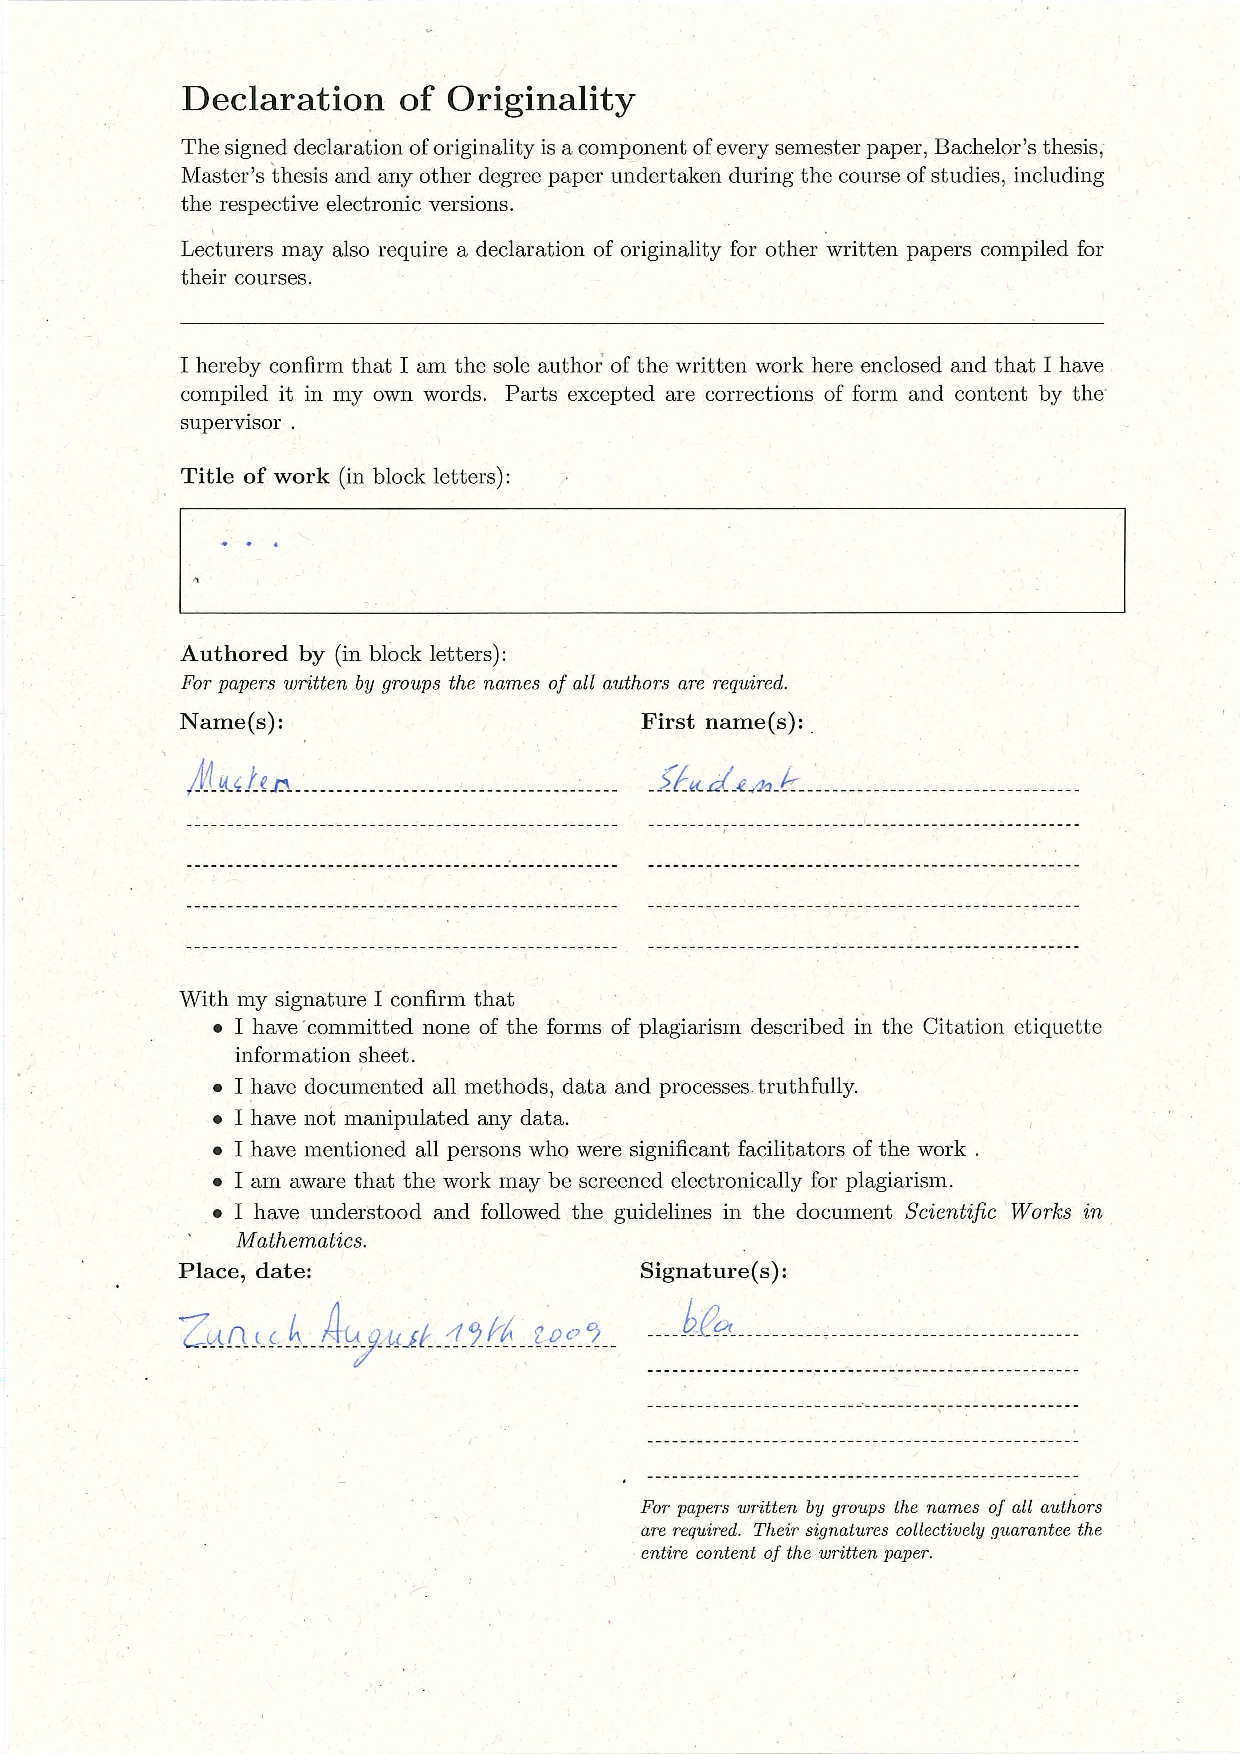
\includepdf[pages={-}, frame=true,scale=1]{misc/confirmation-originality-scan.pdf}
\end{document}


%%% Local Variables:
%%% mode: latex
%%% TeX-master: "MasterThesisSfS"
%%% End:
